% !TeX program = pdflatex
\documentclass[11pt]{amsart}

\usepackage[dvipsnames]{xcolor}
\usepackage{enumitem}
\usepackage{amssymb,graphicx,mathtools,microtype}
\usepackage{nicefrac}
\usepackage{tikz}
\usetikzlibrary{arrows.meta}
\usepackage[margin=1in]{geometry}
\geometry{letterpaper}
\usepackage{etoolbox}
\usepackage[square,longnamesfirst]{natbib}
\usepackage{xurl}
\renewcommand{\bibfont}{\small}
\AtBeginEnvironment{thebibliography}{\raggedbottom}

\theoremstyle{plain}
\newtheorem{theorem}{Theorem}[section]
\newtheorem{proposition}[theorem]{Proposition}
\newtheorem{lemma}[theorem]{Lemma}
\theoremstyle{definition}
\newtheorem{problem}{Problem}[section]
\newtheorem{remark}[theorem]{Remark}

\newcommand{\Z}{\mathbb Z}
\newcommand{\R}{\mathbb R}
\renewcommand{\P}{\mathbb P}
\newcommand{\E}{\mathbb E}
\newcommand{\Var}{\operatorname{Var}}
\newcommand{\drift}{\kappa}
\newcommand{\gauge}{\Psi}
\newcommand{\ind}{\mathbf 1}
\newcommand{\dd}{\,\mathrm d}
\newcommand{\defn}[1]{\textbf{#1}}
\newcommand{\nf}{\nicefrac}
\newcommand{\Rin}{R_{\mathrm{in}}}
\newcommand{\Rout}{R_{\mathrm{out}}}
\newcommand{\Rmom}{R_{\mathrm{mom}}}
\setcounter{secnumdepth}{2}
\numberwithin{equation}{section}

\makeatletter
\patchcmd{\@settitle}{\uppercasenonmath\@title}{\Large}{}{}
\patchcmd{\@setauthors}{\MakeUppercase}{\large}{}{}
\makeatother

\usepackage[citecolor=PineGreen,colorlinks=true,
linkcolor=RoyalBlue,urlcolor=BrickRed]{hyperref}
\hypersetup{pdftitle={Limit shapes for centrally excited walks},
pdfauthor={Ahmed Bou-Rabee, Tuan-Minh Nguyen, Yuval Peres, Arvind Singh}}

\title[Limit shapes for centrally excited walks]{Limit shapes for centrally excited walks}
\author{Ahmed Bou-Rabee}
\address{Department of Mathematics, University of Pennsylvania,
Philadelphia, PA 19104, USA}
\email{ahmedmb@sas.upenn.edu}
\author{Tuan-Minh Nguyen}
\address{School of Mathematics, Monash University,
9 Rainforest Walk, Clayton 3800, Victoria, Australia}
\email{tuanminh.nguyen@monash.edu}
\author{Yuval Peres}
\address{Beijing Institute of Mathematical Sciences and Applications,
Beijing 101408, China}
\email{yperes@bimsa.cn}
\author{Arvind Singh}
\subjclass[2020]{Primary 60K35; Secondary 60G50, 60G42, 31C20}
\keywords{Excited random walk, self-interacting walks, limit shapes,
norms, local times, martingale central limit theorem, law of the iterated
logarithm}
\date{}

\begin{document}

\begin{abstract}
A centrally excited random walk on $\Z^d$ moves like simple random walk, except that its first step from each site has a drift of fixed size toward the origin. Kozma (2007) conjectured that after $n$~steps the visited set approximates a ball with radius of order~$n^{\nf{1}{(d+1)}}$. We prove this in every dimension $d\geq2$ and show that the rescaled numbers of visits converge uniformly to a cone, which is the potential generated by the drift on a ball. The same argument shows that a drift opposite to a subgradient of a norm produces the ball of that norm. In the plane, the outer and inner radii of the visited set differ by at most $n^{\nf16}$ times a power of~$\log n$, and the exponent~$\nf16$ cannot be lowered.
\end{abstract}

\maketitle

\begin{figure}[!b]
\centering
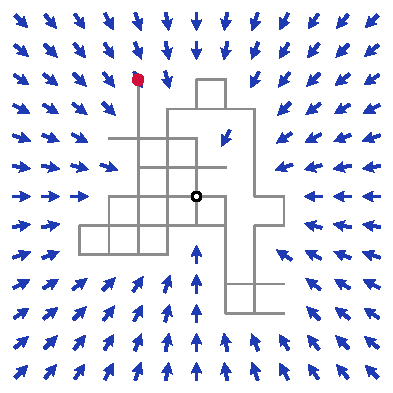
\includegraphics[width=0.5\textwidth]{Figures/first_departure_norms.pdf}
\caption{The walk after $120$~steps, for $d=2$ and $\drift=0.4$: its path (gray), the origin (open circle) and its position (red dot). At each site~$x\neq0$ that it has not yet left, an arrow shows the mean $-\drift x/|x|$ of its first step from~$x$.}
\label{fig:mechanism}
\end{figure}

\section{Introduction}\label{sec:introduction}

Let $d\geq2$ and $0<\drift<1/d$. A \defn{centrally excited random walk} $X_0=0,X_1,X_2,\ldots$ on~$\Z^d$ moves like simple random walk, except that on its first departure from each site~$x\neq0$ it moves to $x\pm e_i$ with probability~$1/(2d)\mp\drift x_i/(2|x|)$ for $1\leq i\leq d$, where $e_1,\ldots,e_d$ is the standard basis of~$\R^d$. Given the path up to that departure, this step has mean~$-\drift x/|x|$, a drift of size~$\drift$ toward the origin (Figure~\ref{fig:mechanism}).

At an Oberwolfach problem session, \citet{Oberwolfach2007} conjectured that the visited set approximates a ball of radius of order~$n^{\nf{1}{(d+1)}}$. We prove this for every $d\geq2$, identify the radius and the uniform limit of the local times, and bound the fluctuations of both. In the plane the inner and outer radii of the visited set fluctuate on the scale~$n^{\nf16}$ up to logarithmic factors; in higher dimensions their fluctuations are bounded by powers of~$\log n$. More generally, a first-departure drift opposite to a subgradient of a norm produces the ball of that norm.

\subsection{The limit shape}\label{sec:shape}

For an integer~$n\geq0$ let
\begin{equation*}
\ell_n(x)\coloneqq\sum_{j=0}^{n-1}\ind_{\{X_j=x\}}
\qquad\text{and}\qquad
A_n\coloneqq\{x:\ell_n(x)>0\}\, .
\end{equation*}
The \defn{local time}~$\ell_n(x)$ is the number of departures from~$x$ before time~$n$, and $A_n$ is the \defn{range}; the set of sites visited by time~$n$ is~$A_{n+1}$. Write $B(y,\rho)$ for the open Euclidean ball of radius~$\rho$ about~$y$ and $\omega_d$ for the volume of~$B(0,1)$, and let
\begin{equation}\label{eq:radius}
r_n\coloneqq\left(\frac{(d+1)n}{2d\drift\omega_d}\right)^{\frac{1}{d+1}}\, ,
\end{equation}
so that the cone $2d\drift(r_n-|v|)_+$ has integral~$n$. Our first theorem says that the range approximates~$B(0,r_n)$ and the local times approximate this cone. 

\begin{theorem}[Limit shape]\label{thm:shape}
Let $d\geq2$ and $0<\drift< \frac1d$. Then, almost surely, the centrally excited random walk has the following properties.
\begin{enumerate}[label=\textup{(\roman*)}]
\item \underline{\emph{Shape}}: for every $0<\eta<1$ and all sufficiently large~$n$,
\begin{equation*}
\{x\in\Z^d:|x|<(1-\eta)r_n\}\subset A_n\subset\{x\in\Z^d:|x|<(1+\eta)r_n\}\, .
\end{equation*}
\item \underline{\emph{Local times}}: as $n\to\infty$,
\begin{equation*}
\frac1{r_n}\max_{x\in\Z^d}\bigl|\ell_n(x)-2d\drift(r_n-|x|)_+\bigr|\longrightarrow0\, .
\end{equation*}
\item \underline{\emph{Recurrence}}: the walk visits every site of~$\Z^d$ infinitely often.
\end{enumerate}
\end{theorem}

\subsection{Fluctuations}\label{sec:fluct-intro}

Replace each site~$x\in A_n$ by the unit cell~$C_x\coloneqq x+[- \frac12, \frac12)^d$, and let $D_n\coloneqq\bigcup_{x\in A_n}C_x$. Define the \defn{inner radius} and the \defn{outer radius} as
\begin{equation}\label{eq:radii}
\Rin(n)\coloneqq\inf_{y\notin D_n}|y|
\qquad\text{and}\qquad
\Rout(n)\coloneqq\max_{0\leq j\leq n}|X_j|\, .
\end{equation}

\begin{theorem}[Fluctuation bounds]\label{thm:fluctuations}
Let $d\geq2$ and $0<\drift<1/d$. For every $p>0$ there exists $C(d,\drift,p)<\infty$ such that, for every integer~$n\geq2$, the following bounds hold simultaneously with probability at least $1-Cn^{-p}$.
\begin{enumerate}[label=\textup{(\roman*)}]
\item \underline{\emph{Radii}}:
\begin{equation*}
\begin{aligned}
|\Rin(n)-r_n|&\leq C\sqrt{r_n\log n}&&\text{and}\quad&\Rout(n)-r_n&\leq C\sqrt{r_n}(\log n)^{\nf52}&&\text{if } d=2\, ,\\
|\Rin(n)-r_n|&\leq C\log n&&\text{and}\quad&\Rout(n)-r_n&\leq C(\log n)^{d+1}&&\text{if } d\geq3\, .
\end{aligned}
\end{equation*}
\item \underline{\emph{Volume}}:
\begin{equation*}
\bigl|r_n^{-1}D_n\mathbin{\triangle}B(0,1)\bigr|
\leq C\begin{dcases}\sqrt{\frac{\log n}{r_n}},&d=2,\\\frac{\log n}{r_n},&d\geq3\end{dcases}\, .
\end{equation*}
\item \underline{\emph{Local times}}:
\begin{equation*}
\max_{x\in\Z^d}\bigl|\ell_n(x)-2d\drift(r_n-|x|)_+\bigr|
\leq C\begin{cases}\sqrt{r_n}(\log n)^{\nf32},&d=2,\\\sqrt{r_n\log n},&d\geq3\end{cases}\, .
\end{equation*}
\end{enumerate}
In particular, these bounds hold for all sufficiently large~$n$ almost surely. 
\end{theorem}

In the plane, $r_n$ has order~$n^{\nf13}$, so part~(i) bounds the deviations of both radii from~$r_n$ by $n^{\nf16}$ times a power of~$\log n$; in higher dimensions it bounds them by a power of~$\log n$. The next theorem shows that the planar exponent~$\nf16$ cannot be lowered and that the local-time bound in part~(iii) has the correct order in $d\geq3$.

\begin{theorem}[Sharpness]\label{thm:sharp}
Let $d\geq2$ and $0<\drift<\nf{1}{d}$, and consider the centrally excited random walk.
\begin{enumerate}[label=\textup{(\roman*)}]
\item \underline{\emph{Radii in the plane}}: let $d=2$. For every $p>0$ there exists $c(\drift,p)>0$ such that, for all sufficiently large~$n$,
\begin{equation}\label{eq:planar-polynomial-lower}
\P\bigl(r_n-\Rin(n)\geq c\sqrt{r_n\log n}\bigr)\geq n^{-p}
\qquad\text{and}\qquad
\P\bigl(\Rout(n)-r_n\geq c\sqrt{r_n\log n}\bigr)\geq n^{-p}\, .
\end{equation}
\item \underline{\emph{Iterated logarithm for the radii in the plane}}: let $d=2$. Almost surely,
\begin{equation}\label{eq:planar-lil-lower}
\limsup_{n\to\infty}\frac{r_n-\Rin(n)}{\sqrt{r_n\log\log n}}\geq\frac1{\sqrt{10\pi\drift}}
\qquad\text{and}\qquad
\limsup_{n\to\infty}\frac{\Rout(n)-r_n}{\sqrt{r_n\log\log n}}\geq\frac1{\sqrt{10\pi\drift}}\, .
\end{equation}
\item \underline{\emph{Local times near the origin}}: there exists $c(d,\drift)>0$ such that, for all sufficiently large~$n$, with probability at least $1-n^{-c}$,
\begin{equation}\label{eq:sharp-bulk}
\max_{\substack{x\in\Z^d\\|x|\leq r_n^{\nf12}}}\bigl|\ell_n(x)-2d\drift(r_n-|x|)\bigr|
\geq c\begin{cases}\sqrt{r_n}\log n,&d=2,\\\sqrt{r_n\log n},&d\geq3\end{cases}\, .
\end{equation}
\item \underline{\emph{Difference of the radii in the plane}}: let $d=2$.
\begin{enumerate}[label=\textup{(\alph*)}]
\item For every $p>0$ there exists $c(\drift,p)>0$ such that, for all sufficiently large~$n$,
\begin{equation}\label{eq:planar-width-polynomial}
\P\bigl(\Rout(n)-\Rin(n)\geq c\sqrt{r_n\log n}\bigr)\geq n^{-p}\, .
\end{equation}
\item Almost surely,
\begin{equation}\label{eq:planar-width-lil}
\limsup_{n\to\infty}\frac{\Rout(n)-\Rin(n)}{\sqrt{r_n\log\log n}}\geq\sqrt{\frac{\pi}{3\drift}}\, .
\end{equation}
\item For every $a\geq0$,
\begin{equation}\label{eq:planar-width-small}
\limsup_{n\to\infty}\P\bigl(\Rout(n)-\Rin(n)\leq a\sqrt{r_n}\bigr)\leq1-\exp\Bigl(-\frac{3\drift a^2}{\pi}\Bigr)\, .
\end{equation}
\end{enumerate}
\end{enumerate}
\end{theorem}

Part~(i) shows that the bound on $|\Rin(n)-r_n|$ in Theorem~\ref{thm:fluctuations}\,(i) is attained, up to the constant, with probability at least~$n^{-p}$. Part~(iv) shows that the planar fluctuations are not only fluctuations of a radius: by~(c), the outer and inner radii differ by more than $a\sqrt{r_n}$ with probability at least $e^{-3\drift a^2/\pi}-o(1)$. Part~(iii) matches the local-time bound of Theorem~\ref{thm:fluctuations}\,(iii) when $d\geq3$; in the plane we show in Section~\ref{sec:lower} that, away from the boundary, the local times deviate from the cone by at most $C\sqrt{r_n}\log n$, so part~(iii) is sharp there as well.

\subsection{Limit shapes for other norms}\label{sec:norms-intro}
The limit shape theorem extends to drifts given by other norms. Let $\gauge$ be a norm with unit ball~$B_\gauge$. Replace $x/|x|$ in the first-departure probabilities by a subgradient~$\xi(x)$ of~$\gauge$ at~$x$, chosen in advance at each site, and assume $\drift\max_i\gauge(e_i)<1/d$. Then the range approximates~$\{\gauge<r_n\}$ and the local times approximate~$2d\drift(r_n-\gauge)_+$, with $|B_\gauge|$ replacing~$\omega_d$ in~\eqref{eq:radius} (Theorem~\ref{thm:norm-shape}).

The theorem includes norms with corners, such as $\|\cdot\|_1$ and~$\|\cdot\|_\infty$, with rates uniform in the choice of subgradients. It also extends to the Minkowski functional of every compact convex set containing the origin in its interior (end of Section~\ref{sec:norms}). Figures~\ref{fig:ranges} and~\ref{fig:profiles} show the range and the local times.

\begin{figure}[t]
\centering
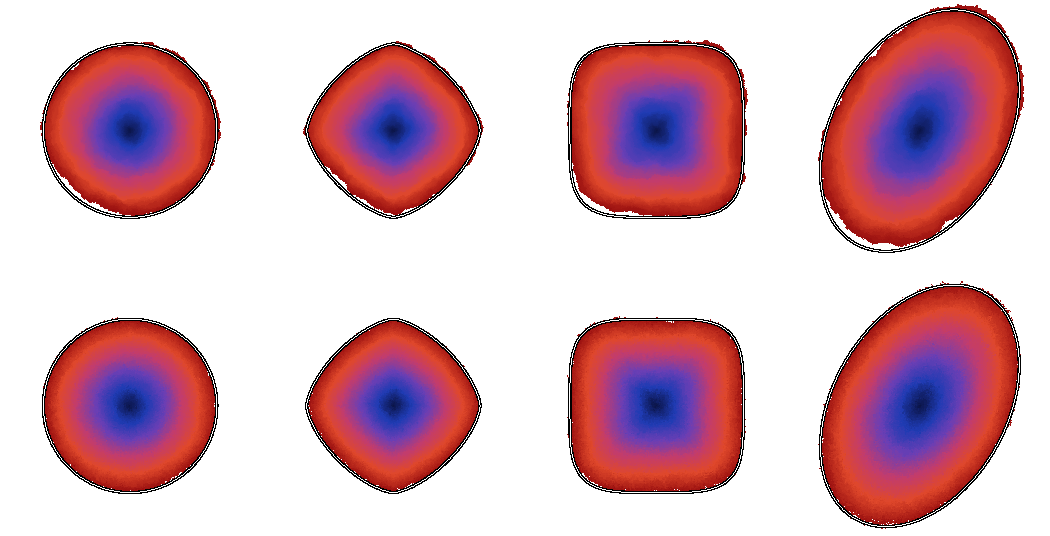
\includegraphics[width=\textwidth]{Figures/shapes_ranges.pdf}
\caption{Ranges $r_n^{-1}A_n$ for the Euclidean, $\ell^{3/2}$, $\ell^4$ and elliptical norms (left to right), at $n=10^9$. Top: $d=2$, $\drift=0.4$; bottom: $x_3=0$ sections for $d=3$, $\drift=0.25$. The unit balls are outlined and the blue-to-red colors show $(t_x/n)^{\nf{1}{(d+1)}}$, with $t_x$ the first-departure time.}
\label{fig:ranges}
\end{figure}
\begin{figure}[t]
\centering
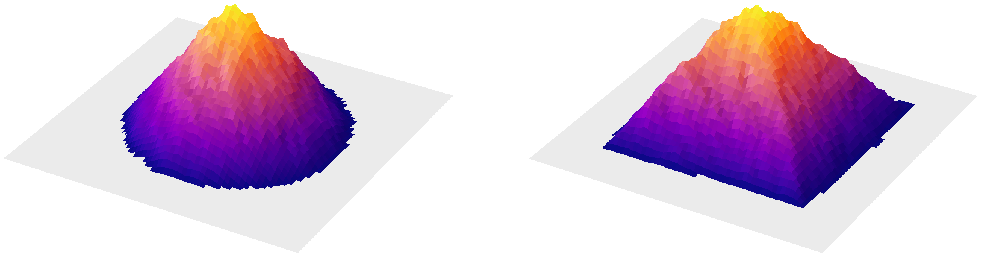
\includegraphics[width=\textwidth]{Figures/shapes_localtimes.pdf}
\caption{Local times $\ell_n(x)/(2d\drift r_n)$ over $x/r_n$ for the Euclidean norm (left) and $\ell^\infty$ (right): $d=2$, $n=10^{10}$, $\drift=0.4$. }
\label{fig:profiles}
\end{figure}



\subsection{Strategy and key ideas}\label{sec:strategy}

The proof compares the local times with an explicit potential. Dynkin's formula for the Green function with pole~$y$ writes~$\ell_n(y)$ as a sum over the first departures, each weighted by the inner product of its drift with the gradient of the Green function, plus a martingale and a smaller error. The continuum version of this sum is a potential: for a bounded measurable set~$D\subset\R^d$ and $y\in\R^d$, let
\begin{equation}\label{eq:potential-intro}
U_D(y)\coloneqq\frac{2\drift}{\omega_d}\int_D\frac{v}{|v|}\cdot\frac{v-y}{|v-y|^d}\dd v
\end{equation}
be the potential generated by the vector field~$-\drift v/|v|$ on~$D$. Integration along the rays from~$y$ shows that the potential of a ball is a cone: for every $\rho>0$ and every $y\in\R^d$,
\begin{equation}\label{eq:ballpotential-euclid}
U_{B(0,\rho)}(y)=2d\drift(\rho-|y|)_+\, .
\end{equation}
Replacing $v/|v|$ by~$\nabla\gauge(v)$ gives the cone $2d\drift(\rho-\gauge(y))_+$ for a ball of the norm (Lemma~\ref{lem:ballpotential}).

So Dynkin's formula compares~$\ell_n$ with~$U_{D_n}$, up to a martingale and a smaller error. Near the boundary of the range, the martingale error bound can be larger than the local times and the potential, so this comparison alone need not locate the boundary. We use two further facts. Local times vanish outside the range, and the walk can reach a distant site only by crossing the intervening region against its first-departure drift. The main comparison is at a contact point: a point~$y_0$ that lies both on the boundary of the largest ball about the origin contained in~$D_n$ and in the closure of a cell disjoint from~$D_n$. The local time vanishes on that cell, so the potential at~$y_0$ is small, while every point of~$D_n$ outside the ball contributes nonnegatively to it.
\begin{enumerate}[label=\arabic*.,leftmargin=*]
\item \emph{Local times and the potential} (Section~\ref{sec:local}). Freedman's inequality controls the martingales in Dynkin's formula uniformly over sites. Replacing the sum over first departures by~$U_{D_n}$ costs $O(\log n)$, also for norms with corners; convexity controls the variation of the subgradients across a cell (Lemma~\ref{lem:cell}).
\item \emph{Crossing and coarse bounds} (Section~\ref{sec:coarse}). Let $\tau_R$ be the time at which the walk leaves the ball of the norm with radius~$R$. Until~$\tau_R$, and until one of the martingales in Dynkin's formula exceeds~$R$ in absolute value, Dynkin's formula bounds each local time by~$CR$, and hence the elapsed time by~$CR^{d+1}$; Freedman's inequality then shows that the martingales are unlikely to exceed~$R$ before~$\tau_R$. At time~$\tau_R$, the comparison at the contact point and the crossing argument show that the range contains all sites of a ball of radius~$cR$, and that the local times have order~$R$ on the concentric ball of half this radius; so $\tau_R\geq cR^{d+1}$, and the coarse bounds at time~$n$ follow (Proposition~\ref{prop:coarse}). For a norm with corners, we cross in the direction~$u$ from the nearest point of a ball of the norm to the visited site farthest from this ball in Euclidean distance: at every visited site~$y$ at which $u\cdot y$ is close to its maximum over the visited sites, every subgradient of~$\gauge$ has positive inner product with~$u$.
\item \emph{The limit shape} (Section~\ref{sec:norms}). Let $b$ be the radius of the largest ball of the norm about the origin contained in~$D_n$. By convexity, every point~$v$ of~$D_n$ outside this ball contributes at least $c(\gauge(v)-b)r_n^{-d}$ to the potential at the contact point. Dynkin's formula at the center of the adjacent cell bounds this potential by the martingale there, and Dynkin's formula for the square of the Green function bounds the bracket of that martingale in terms of the local time at its pole, which vanishes (Lemma~\ref{lem:contact}). So the part of~$D_n$ outside the ball has small potential, which gives the cone for the local times, and the martingale obtained from~$|X_n|^2$ gives $b\approx r_n$. The local times outside $\{\gauge<r_n\}$ are then small, and the crossing argument shows that no visited site lies far from $\{\gauge\leq r_n\}$.
\item \emph{The inner radius} (Section~\ref{sec:contact}). For the Euclidean norm, every point~$v$ of~$D_n$ outside the inner ball contributes at least $c|v-y_0|^{2-d}/r_n$ to the potential at the contact point~$y_0$, a bound that does not vanish near the boundary of the ball. With Lemma~\ref{lem:contact}, this bounds the volume of~$D_n$ outside the ball and sharpens the inner-radius estimate (Proposition~\ref{prop:inner}).
\item \emph{The outer radius} (Section~\ref{sec:outer}). We evaluate the potential at points beyond the outer radius, where the local time vanishes. Points of~$D_n$ near the outer sphere contribute negatively to this potential. The curvature of the sphere bounds the positive contributions by an integral of $|v-y|^{2-d}/|v|$ over the part of~$D_n$ outside the inner ball, which we bound by integrating the potential along rays when $d\geq3$ and by the volume bound of Section~\ref{sec:contact} when $d=2$. So little of~$D_n$ lies near the outer sphere. These volume bounds control the local times outside the inner ball, and the crossing argument gives the outer-radius bound (Proposition~\ref{prop:stronger-outer}). The same estimates and the maximum principle for the potential of this part of~$D_n$ give the uniform local-time bound.
\end{enumerate}
The cone determines the limits of the brackets of the martingales in Dynkin's formula and of the martingale obtained from~$|X_n|^2$, so the martingale central limit theorem and the law of the iterated logarithm give the limit laws of Section~\ref{sec:sharp}. The lower bounds need deviations of about $(\log n)^{\nf12}$ standard deviations, which we obtain from exponential martingales: the martingale obtained from~$|X_n|^2$ controls the planar radii, and many weakly correlated martingales in Dynkin's formula control the largest deviation of the local times near the origin. The difference of the radii is controlled by the vector martingale $X_n+\drift\sum_{x\in A_n}x/|x|$: the vectors $x/|x|$ cancel inside the inner disk, so fluctuations of order~$\sqrt n$ of this martingale force fluctuations of order~$\sqrt{r_n}$ of the difference of the radii, and its two-dimensional Gaussian limit gives the bound in Theorem~\ref{thm:sharp}\,(iv)(c). Figure~\ref{fig:dependence} records the dependencies.

\begin{figure}[t]
\centering
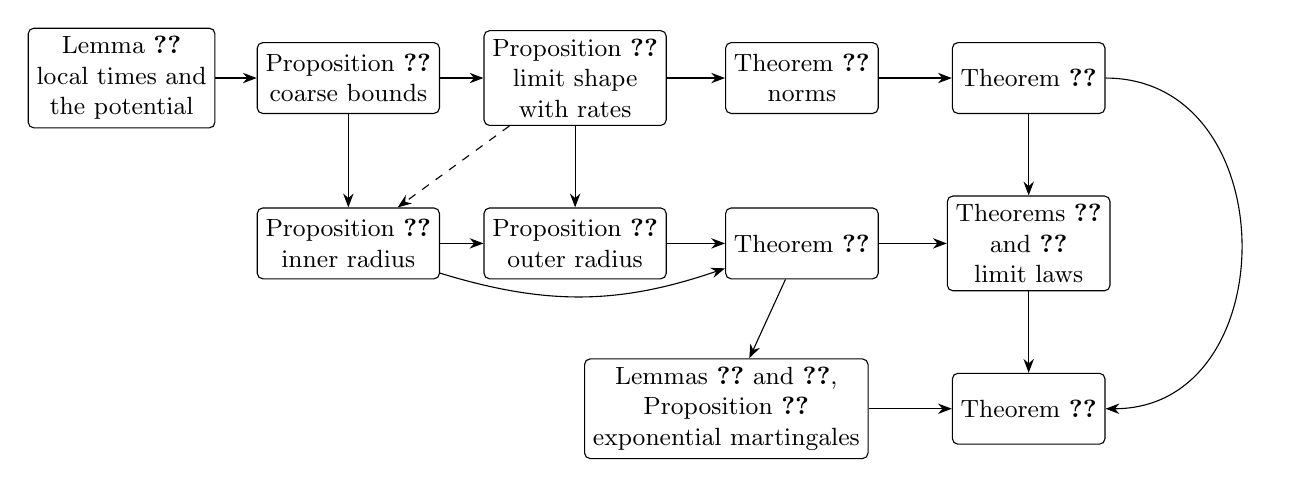
\begin{tikzpicture}[x=0.96cm,y=1cm,
  box/.style={draw,rounded corners=2pt,align=center,font=\small,
    inner sep=3pt,minimum height=0.9cm},
  arr/.style={-{Stealth[length=5pt]},thin}]
\node[box] (L) at (0,0) {Lemma~\ref{lem:local}\\ local times and\\ the potential};
\node[box] (P3) at (3,0) {Proposition~\ref{prop:coarse}\\ coarse bounds};
\node[box] (P4) at (6,0) {Proposition~\ref{prop:norm-shape}\\ limit shape\\ with rates};
\node[box] (TN) at (9,0) {Theorem~\ref{thm:norm-shape}\\ norms};
\node[box] (TA) at (12,0) {Theorem~\ref{thm:shape}};
\node[box] (P5) at (3,-2.1) {Proposition~\ref{prop:inner}\\ inner radius};
\node[box] (P6) at (6,-2.1) {Proposition~\ref{prop:stronger-outer}\\ outer radius};
\node[box] (TB) at (9,-2.1) {Theorem~\ref{thm:fluctuations}};
\node[box] (S8) at (12,-2.1) {Theorems~\ref{thm:moment-fluctuations}\\ and~\ref{thm:site-fluctuations}\\ limit laws};
\node[box] (S9) at (8,-4.2) {Lemmas~\ref{lem:exp-deviation} and~\ref{lem:separated-brackets},\\ Proposition~\ref{prop:bulk-profile}\\ exponential martingales};
\node[box] (TC) at (12,-4.2) {Theorem~\ref{thm:sharp}};
\draw[arr] (L) -- (P3);
\draw[arr] (P3) -- (P4);
\draw[arr] (P4) -- (TN);
\draw[arr] (TN) -- (TA);
\draw[arr] (P3) -- (P5);
\draw[arr] (P5) -- (P6);
\draw[arr] (P6) -- (TB);
\draw[arr] (P5) to[bend right=18] (TB);
\draw[arr,dashed] (P4) -- (P5);
\draw[arr] (P4) -- (P6);
\draw[arr] (TA) -- (S8);
\draw[arr] (TB) -- (S8);
\draw[arr] (TB) -- (S9);
\draw[arr] (S8) -- (TC);
\draw[arr] (S9) -- (TC);
\draw[arr] (TA.east) to[out=0,in=0,looseness=1.4] (TC.east);
\end{tikzpicture}
\caption{Dependencies among the main results. A solid arrow means that a result is used; a dashed arrow means that estimates from Section~\ref{sec:norms} are used.}
\label{fig:dependence}
\end{figure}

The local times play the role of the odometer of the divisible sandpile, which \citet{LevinePeres2009} compared with an explicit potential. Martingales with a pole at an unvisited site, and separate estimates that rule out thin tentacles, also appear in the bounds of~\citet*{JerisonLevineSheffield2012,JerisonLevineSheffield2013} for internal diffusion-limited aggregation. Our logarithmic lower bounds use the inner/outer deviation dichotomy of~\citet[Proposition~1.2]{AsselahGaudilliere2014}.

\subsection{Related work}\label{sec:related}

\citet{Kozma2013} reported recurrence of the walk excited to the center, citing unpublished work from 2006. \citet*{DemboHuangSidoravicius2014} described the manuscript of~\citet{Kozma2006CentrallyExcited} for a related walk in $d\geq3$, with drift~$-\drift x/\|x\|_1$ at the first visit to a site having an unvisited neighbor; \citet*{DemboHuangSidoravicius2014Growing} cited it for recurrence in every dimension. We take the name centrally excited random walk from the title of that manuscript. The drift of its walk has a Euclidean length that depends on the direction, whereas our drift has length~$\drift$. \citet*{BenjaminiDuminilCopinKozmaLucas2020} also recorded the predicted radius~$n^{\nf{1}{(d+1)}}$.

For the excited random walk with first-visit drift in a fixed direction, \citet*{BenjaminiWilson2003} proved transience in $d\geq2$ and positive lower speed in $d\geq4$. \citet{Kozma2003Speed,Kozma2005Speed} obtained positive lower speed in $d=3$ and $d=2$, and \citet{BerardRamirez2007} proved laws of large numbers and central limit theorems. \citet*{MenshikovPopovRamirezVachkovskaia2012} extended positive-speed results to uniformly elliptic walks with bounded jumps and uniformly positive first-visit drift in a fixed direction and zero drift at later visits. \citet{Zerner2005,Zerner2006} gave recurrence/transience criteria on~$\Z$ and strips for walks with multiple cookies. \citet*{AmirBenjaminiKozma2008} proved recurrence for a walk in the upper half of~$\Z^3$ that steps down at new sites. See~\citet{KosyginaZerner2013} for a survey.

The radius~$n^{\nf{1}{(d+1)}}$ and range size~$n^{\nf{d}{(d+1)}}$ are also predicted for once-reinforced walks with strong reinforcement~\citep{Beffara2011,ElboimKozma2026}, and supported by simulations~\citep{FosterGrassbergerPaczuski2009}; related predictions for self-attracting walks appear in~\citet{OrdemannBerkolaikoHavlinBunde2000,OrdemannEtAl2001}. For once-reinforced random walk on~$\Z^d$ with $d\geq2$, \citet{BouRabeePeres2026ORRW} proved the lower bound~$cn^{\nf{d}{(d+1)}}$ on the expected range for every reinforcement parameter. The matching upper bound and limit shape remain conjectural. See~\citet{Pemantle2007} for reinforced processes.

\citet{DemboGroismanHuangSidoravicius2021} proved an averaging principle and shape theorem for growth models motivated by origin-excited and once-reinforced walks. Their simulations with inward first steps along a coordinate of largest absolute value or along all coordinates produced squares and diamonds. Our norm theorem proves these shapes for first-departure drifts opposite to subgradients of~$\|\cdot\|_\infty$ and~$\|\cdot\|_1$. For related continuum growth models, \citet*{DemboYang2025Flow,DemboYang2025KPZ} obtained limits described by geometric flow and regularized Kardar--Parisi--Zhang equations.

Internal diffusion-limited aggregation~\citep{LawlerBramsonGriffeath1992} and rotor-router aggregation~\citep{LevinePeres2009} have Euclidean ball limit shapes. The former has radius fluctuations of order at most $\log r$ in the plane and $(\log r)^{\nf12}$ in higher dimensions~\citep{JerisonLevineSheffield2012,JerisonLevineSheffield2013,AsselahGaudilliere2013,AsselahGaudilliere2013Polynomial}, and its rescaled fluctuations approach a variant of the Gaussian free field~\citep{JerisonLevineSheffield2014}. For the centrally excited walk, Theorem~\ref{thm:sharp} gives much larger planar fluctuations of the radii and of their difference; the fixed-site covariance in Theorem~\ref{thm:site-fluctuations} is again expressed through the Green function. See~\citet*{LevinePeres2017} for aggregation models.

For Eulerian walkers~\citep{PriezzhevDharDharKrishnamurthy1996}, simulations suggested a circular planar range of radius of order~$n^{\nf13}$ after $n$~steps~\citep{KapriDhar2009}. \citet*{FlorescuLevinePeres2016} proved that every simple rotor walk on~$\Z^d$ visits at least $cn^{\nf{d}{(d+1)}}$ sites in $n$~steps. For clockwise planar rotors with independent uniform initial states, \citet*{BouRabeePeres2026} proved convergence of the rescaled range to a deterministic compact convex set; whether it is a disk remains open.

\subsection{Notation and conventions}\label{sec:notation}

\begin{itemize}
\item The Euclidean norm is $|x|$, and $\|x\|_p$ is the $\ell^p$~norm for $1\leq p\leq\infty$. The cardinality of a set~$A\subset\Z^d$ is~$|A|$, and the Lebesgue measure of a set~$D\subset\R^d$ is~$|D|$. The symmetric difference is~$\triangle$, and $t_+\coloneqq\max\{t,0\}$ and $s\wedge t\coloneqq\min\{s,t\}$.
\item Let $u_x\coloneqq x/|x|$ for $x\in\R^d\setminus\{0\}$ and $u_0\coloneqq0$, and let $\xi(0)\coloneqq0$.
\item The letters $c>0$ and $C>0$ denote constants depending only on $d$, $\drift$ and the exponent~$p$ of the failure probability under discussion, and in Sections~\ref{sec:norm-setup}--\ref{sec:norms} also on the norm~$\gauge$, but not on the choice of the subgradients~$\xi(x)$; they may change from line to line. Every further dependence is stated, and a subscript on~$O$, as in~$O_y$, means that the implied constant also depends on~$y$. We write $a_n\asymp b_n$ if $c\leq a_n/b_n\leq C$.
\item The $\sigma$-field generated by $X_0,\ldots,X_j$ is~$\mathcal F_j$. For martingales $Z_1$ and~$Z_2$, the brackets $\langle Z_1\rangle_n$ and~$\langle Z_1,Z_2\rangle_n$ are the predictable quadratic variation and covariation through time~$n$.
\item The indicator that the step at time~$j$ is a first departure is $I_j\coloneqq\ind_{\{X_j\notin A_j\}}$, so that $\E(X_{j+1}-X_j\mid\mathcal F_j)=-\drift I_j\xi(X_j)$, where $\xi(x)=u_x$ for the Euclidean norm.
\item The function~$\widetilde\ell_n$ on~$\R^d$ equals $\ell_n(x)$ on~$C_x$ for every $x\in\Z^d$; it vanishes off~$D_n$.
\item All estimates concern integers~$n\geq2$, so that $\log n>0$. In a statement that holds with probability at least $1-Cn^{-p}$ for all sufficiently large~$n$, enlarging~$C$ makes it hold for every $n\geq2$.
\end{itemize}

\subsection{Lean formalization}\label{ssec:formalization}
Every labeled theorem, lemma, proposition and corollary of this paper has been formalized in Lean~4. The formalization builds on Mathlib.  No proof uses \texttt{sorry} or an axiom beyond the three standard axioms \texttt{propext}, \texttt{Classical.choice} and \texttt{Quot.sound}. The development is at \url{https://github.com/nitromannitol/Centrally-Excited-Random-Walk}.

\subsection*{Use of artificial intelligence}
The authors developed the main ideas of this work and directed its mathematical development. Throughout the project, the authors used large language models as research assistants: to explore specific questions arising in the proofs, to check the arguments and the cited results, and to audit drafts of the paper. The exposition, the simulations and the figures were produced with AI agents, primarily Claude (Anthropic), under the close supervision of the authors. The authors take responsibility for the mathematical content and presentation of the paper.

\subsection*{Acknowledgments}
The research of Y. Peres was supported by the National Natural Science Foundation of China grant RFIS-W2531011.

\subsection*{Earlier versions and related models}
This paper develops the results of \citet{BouRabeePeres2026CERW}. The proof of the coarse bounds in Section~\ref{sec:coarse} uses the stopping argument of \citet{Singh2026}, who allowed arbitrary first-departure laws with mean $-\drift x/|x|$ at every nonzero site and a symmetric first-departure law at the origin. \citet{Nguyen2026} considered first-departure laws that favor the neighbors decreasing the $\ell^1$ distance to the origin, and proved convergence in probability, in Hausdorff distance, of the rescaled visited set to an explicit $\ell^1$ ball in every dimension $d\geq2$.

\section{Drifts given by a norm}\label{sec:norm-setup}

In this section we give the precise setting for a drift opposite to a subgradient of a norm and state the limit shape theorem in this setting, Theorem~\ref{thm:norm-shape}, of which Theorem~\ref{thm:shape} is the Euclidean case. We also prove the identity for the potential of a ball of the norm on which its proof rests (Lemma~\ref{lem:ballpotential}). Sections~\ref{sec:local}--\ref{sec:norms} work in this setting and prove Theorem~\ref{thm:norm-shape} at the end of Section~\ref{sec:norms}.

Let $\gauge$ be a norm on~$\R^d$ and let $B_\gauge$ be its unit ball. A \defn{subgradient} of~$\gauge$ at~$x\in\R^d$ is a vector $\xi\in\R^d$ such that $\gauge(y)\geq\gauge(x)+\xi\cdot(y-x)$ for every $y\in\R^d$, and $\partial\gauge(x)$ is the set of subgradients at~$x$; if $\gauge$ is differentiable at~$x$, then $\partial\gauge(x)=\{\nabla\gauge(x)\}$. At each site~$x\neq0$ fix $\xi(x)\in\partial\gauge(x)$, with coordinates~$\xi_i(x)$. The \defn{centrally excited random walk with norm~$\gauge$} moves like simple random walk, except that on its first departure from each site~$x\neq0$ it moves to $x\pm e_i$ with probability
\begin{equation}\label{eq:kernel}
\frac1{2d}\mp\frac\drift2\xi_i(x)
\qquad\text{for } 1\leq i\leq d\, .
\end{equation}
We assume that
\begin{equation}\label{eq:ellipticity}
\drift\max_{1\leq i\leq d}\gauge(e_i)<\frac1d\, .
\end{equation}
Every $\xi\in\partial\gauge(x)$ satisfies Euler's relation $\xi\cdot x=\gauge(x)$, so the definition of a subgradient gives
\begin{equation}\label{eq:convexity}
\xi\cdot y\leq\gauge(y)\qquad\text{for every }y\in\R^d\, ,
\end{equation}
with equality at $y=x$. Hence $|\xi_i(x)|\leq\gauge(e_i)$, and~\eqref{eq:ellipticity} makes the probabilities~\eqref{eq:kernel} positive. The step at the first departure from~$x$ has conditional mean~$-\drift\xi(x)$, whose inner product with~$x$ is $-\drift\gauge(x)<0$. The Euclidean norm, with $\xi(x)=x/|x|$, gives the walk of Section~\ref{sec:introduction}, and then~\eqref{eq:ellipticity} reads $\drift<\nf1d$. Let
\begin{equation}\label{eq:radius-norm}
r_n\coloneqq\left(\frac{(d+1)n}{2d\drift|B_\gauge|}\right)^{\nf{1}{(d+1)}}\, ,
\end{equation}
which is~\eqref{eq:radius} when $\gauge$ is the Euclidean norm; the cone $2d\drift(r_n-\gauge(v))_+$ has integral~$n$ over~$\R^d$.

In Sections~\ref{sec:norm-setup}--\ref{sec:norms}, $\gauge$ is a norm, $\drift>0$ satisfies~\eqref{eq:ellipticity}, $r_n$ is given by~\eqref{eq:radius-norm}, and $U_D$ is the potential~\eqref{eq:potential-norm} defined below; at a point~$v\in\R^d$, $\nabla\gauge(v)$ is the gradient, which exists for almost every~$v$. Let $\Lambda_\gauge\coloneqq\max_{|u|=1}\gauge(u)$ and $c_\gauge\coloneqq\min_{|u|=1}\gauge(u)$; by~\eqref{eq:convexity}, every subgradient~$\xi$ of~$\gauge$ satisfies $|\xi|\leq\Lambda_\gauge$. In Sections~\ref{sec:contact}--\ref{sec:lower}, $\gauge$ is the Euclidean norm, so that $\xi(x)=u_x$, $r_n$ is given by~\eqref{eq:radius}, and $U_D$ is the potential~\eqref{eq:potential-intro}.

\begin{theorem}[Limit shape for a norm]\label{thm:norm-shape}
Let $d\geq2$, let $\gauge$ be a norm on~$\R^d$, let $\xi(x)\in\partial \gauge(x)$ be chosen at the sites $x\in\Z^d\setminus\{0\}$, let $\drift>0$ satisfy~\eqref{eq:ellipticity}, and let $r_n$ be as in~\eqref{eq:radius-norm}. Then, almost surely, the centrally excited random walk with norm~$\gauge$ has the following properties.
\begin{enumerate}[label=\textup{(\roman*)}]
\item \underline{\emph{Shape}}: for every $0<\eta<1$ and all sufficiently large~$n$,
\begin{equation*}
\{x\in\Z^d:\gauge(x)<(1-\eta)r_n\}\subset A_n\subset\{x\in\Z^d:\gauge(x)<(1+\eta)r_n\}\, .
\end{equation*}
\item \underline{\emph{Local times}}: as $n\to\infty$,
\begin{equation*}
\frac1{r_n}\max_{x\in\Z^d}\bigl|\ell_n(x)-2d\drift(r_n-\gauge(x))_+\bigr|\longrightarrow0\, .
\end{equation*}
\item \underline{\emph{Recurrence}}: the walk visits every site of~$\Z^d$ infinitely often.
\end{enumerate}
\end{theorem}

Proposition~\ref{prop:norm-shape} gives rates: for every $p>0$ there is a constant $C(d,\drift,\gauge,p)$, not depending on the choice of~$\xi$, such that with probability at least $1-Cn^{-p}$ the maximum in part~(ii) is at most $Cr_n^{\nf56}(\log n)^{\nf16}$ if $d=2$ and $Cr_n^{\nf{d}{(d+1)}}(\log n)^{\nf{1}{(d+1)}}$ if $d\geq3$, and the inclusions of part~(i) hold with $\eta r_n$ replaced by $\log n$ times this bound on the maximum. Part~(i) gives $|A_n|/r_n^d\to|B_\gauge|$, and for the Euclidean norm Theorem~\ref{thm:fluctuations} gives smaller error bounds.

\subsection{The potential of a norm ball}\label{sec:ballpotential}

For a norm~$\gauge$, the potential~\eqref{eq:potential-intro} is defined with the gradient of~$\gauge$ in place of~$v/|v|$: for a bounded measurable set~$D\subset\R^d$ and $y\in\R^d$, let
\begin{equation}\label{eq:potential-norm}
U_D(y)\coloneqq\frac{2\drift}{\omega_d}\int_D\nabla\gauge(v)\cdot\frac{v-y}{|v-y|^d}\dd v
\end{equation}
be the potential generated by the vector field~$-\drift\nabla\gauge$ on~$D$.

For every Lipschitz function~$f$ with compact support and every $y\in\R^d$,
\begin{equation}\label{eq:gradient-identity}
\int_{\R^d}\nabla f(v)\cdot\frac{v-y}{|v-y|^d}\dd v=-d\omega_df(y)\, .
\end{equation}
To prove it, write $v=y+tu$ with $t>0$ and $|u|=1$, so that $(v-y)|v-y|^{-d}\dd v=u\dd t\dd S(u)$, where $\dd S$ is surface measure on the unit sphere. By Rademacher's and Fubini's theorems, for almost every~$u$ the Lipschitz function $t\mapsto f(y+tu)$ has derivative $\nabla f(y+tu)\cdot u$ for almost every $t>0$; this function vanishes for large~$t$, so its derivative integrates to $-f(y)$ over $t>0$, and the unit sphere has area $d\omega_d$.

\begin{lemma}[The potential of a norm ball]\label{lem:ballpotential}
Let $\gauge$ be a norm, let $\rho>0$, and let $y\in\R^d$. Then
\begin{equation}\label{eq:ballpotential}
U_{\{\gauge<\rho\}}(y)=2d\drift(\rho-\gauge(y))_+\, .
\end{equation}
\end{lemma}

\begin{proof}
The set $\{\gauge<\rho\}$ is bounded, and $\{\gauge=\rho\}$ has measure zero because $\gauge$ is homogeneous, so $\nabla(\rho-\gauge)_+=-\ind_{\{\gauge<\rho\}}\nabla \gauge$ almost everywhere. Applying~\eqref{eq:gradient-identity} to the Lipschitz function $f=(\rho-\gauge)_+$, which has compact support, proves the lemma.
\end{proof}

For the Euclidean norm, Lemma~\ref{lem:ballpotential} is the identity~\eqref{eq:ballpotential-euclid}.

\section{Local times and the potential}\label{sec:local}

In this section we prove Lemma~\ref{lem:local}, which compares the local times with the potential~$U_{D_n}$. Dynkin's formula expresses each local time as~$U_{D_n}$ minus a martingale, up to an error term. We bound the bracket of this martingale by a weighted sum of the local times, and use convexity to bound the error from replacing the subgradients~$\xi(x)$ chosen at the sites by the gradient~$\nabla\gauge$ on the cells (Lemma~\ref{lem:cell}).

\begin{lemma}\label{lem:local}
Let $p>0$. There exists $C(d,\drift,\gauge,p)<\infty$ such that, for every integer~$n\geq2$, with probability at least $1-Cn^{-p}$, every $y\in\R^d$ with $|y|\leq2n$ satisfies
\begin{equation}\label{eq:approx}
|\widetilde\ell_n(y)-U_{D_n}(y)|\leq C\log n+C\begin{cases}\bigl(\max_x\ell_n(x)\bigr)^{\nf12}\log n,&d=2,\\\bigl(\max_x\ell_n(x)\log n\bigr)^{\nf12},&d\geq3\end{cases}\, .
\end{equation}
\end{lemma}

Once $\max_x\ell_n(x)\leq Cr_n$, as on the event of Proposition~\ref{prop:coarse}, the right side of~\eqref{eq:approx} is at most $C\sqrt{r_n}\log n=o(r_n)$.

\subsection{Dynkin's formula for the local times}\label{sec:dynkin}

Let $\Delta f(x)\coloneqq(2d)^{-1}\sum_{|e|=1}(f(x+e)-f(x))$, summed over the unit vectors $e\in\Z^d$, be the discrete Laplacian. For $d=2$, let $g$ be the potential kernel of simple random walk, normalized by $g(0)=0$. For $d\geq3$, let $g\coloneqq-G$, where the Green function~$G(x)$ is the expected number of visits to~$x$ by simple random walk from the origin. In both cases $\Delta g=\ind_{\{0\}}$; for $d=2$ see \citet*[Proposition~4.4.2]{LawlerLimic2010}. By \citet[Theorems~4.3.1 and~4.4.4]{LawlerLimic2010}, as $|x|\to\infty$,
\begin{equation}\label{eq:kernel-asymptotics}
g(x)=\begin{dcases}
\frac2\pi\log|x|+c_g+O(|x|^{-2}),&d=2,\\
-\frac{2}{(d-2)\omega_d}|x|^{2-d}+O(|x|^{-d}),&d\geq3
\end{dcases}\, ,
\end{equation}
where $c_g$ is a constant. Let $\bar\nabla g(x)$ be the vector with coordinates $(g(x+e_i)-g(x-e_i))/2$ for $1\leq i\leq d$. Then
\begin{equation}\label{eq:gradient}
\bar\nabla g(x)=\frac2{\omega_d}\frac{x}{|x|^d}+O(|x|^{-d})
\quad\text{and}\quad
|g(x+e)-g(x)|\leq C(1+|x|)^{1-d}\, ,
\end{equation}
the first for $x\neq0$, the second for every $x\in\Z^d$ and every unit vector $e\in\Z^d$; see \citet[Corollaries~4.3.3 and~4.4.5]{LawlerLimic2010}.

For $f\colon\Z^d\to\R$ with bounded nearest-neighbor increments, let
\begin{equation*}
\mathcal M^f_t\coloneqq f(X_t)-f(X_0)-\sum_{j<t}\E\bigl(f(X_{j+1})-f(X_j)\bigm|\mathcal F_j\bigr)
\end{equation*}
be the martingale in Dynkin's formula for~$f$. By~\eqref{eq:kernel}, the conditional expectation in the sum is $\Delta f(X_j)-\drift I_j\xi(X_j)\cdot\bar\nabla f(X_j)$, with $\bar\nabla f$ defined like~$\bar\nabla g$. For $y\in\Z^d$ write $g_y\coloneqq g(\cdot-y)$ and $\mathcal M^y\coloneqq\mathcal M^{g_y}$. Since $\Delta g_y=\ind_{\{y\}}$ and each site of~$A_n$ has its first departure before time~$n$,
\begin{equation}\label{eq:dynkin}
\ell_n(y)=g(X_n-y)-g(-y)
+\drift\sum_{x\in A_n}\xi(x)\cdot\bar\nabla g(x-y)-\mathcal M_n^y\, .
\end{equation}
The difference $g(X_n-y)-g(-y)$ is $O(\log n)$ for $d=2$ and $O(1)$ for $d\geq3$, uniformly over $y\in\Z^d$ with $|y|\leq3n$. By~\eqref{eq:gradient}, the increments of~$\mathcal M^y$ are bounded, and a departure from~$x$ adds at most $C(1+|x-y|)^{2-2d}$ to the bracket of~$\mathcal M^y$; so, for every integer $t\geq0$,
\begin{equation}\label{eq:bracket}
\langle\mathcal M^y\rangle_t\leq C\sum_{j<t}(1+|X_j-y|)^{2-2d}\, .
\end{equation}

\begin{lemma}\label{lem:freedman}
Let $p>0$. There exists $C(p)<\infty$ such that the following holds for every integer~$n\geq2$ and every real martingale~$Z$ whose increments have absolute value at most~$1$: with probability at least $1-Cn^{-p}$,
\begin{equation}\label{eq:freedman}
|Z_n-Z_0|\leq C\bigl(\sqrt{\langle Z\rangle_n\log n}+\log n\bigr)\, .
\end{equation}
\end{lemma}

\begin{proof}
For $0\leq i\leq\log_2n+1$, \citet*[Theorem~1.6]{Freedman1975} bounds the probability that $\langle Z\rangle_n\leq2^i$ and $|Z_n-Z_0|>C(p)(\sqrt{2^i\log n}+\log n)$ by $2n^{-p-1}$. Since $\langle Z\rangle_n\leq n$, a union bound over these $O(\log n)$ values of~$i$ proves~\eqref{eq:freedman}.
\end{proof}

We apply Lemma~\ref{lem:freedman} to constant multiples of possibly stopped martingales, with union bounds over polynomially many deterministic sites; the resulting estimates then hold also at sites that depend on the path. In particular, for every $p>0$, with probability at least $1-Cn^{-p}$, simultaneously for all $y\in\Z^d$ with $|y|\leq3n$,
\begin{equation}\label{eq:localmart}
|\mathcal M_n^y|\leq C\bigl(\sqrt{\langle\mathcal M^y\rangle_n\log n}+\log n\bigr)\, .
\end{equation}

Let $\mu$ be the distributional Laplacian of~$\gauge$ on~$\R^d$, so that $\int\phi\dd\mu=\int \gauge(v)\sum_{i=1}^d\partial_i^2\phi(v)\dd v=-\int\nabla\gauge\cdot\nabla\phi$ for every smooth compactly supported function~$\phi$ on~$\R^d$, and hence, by approximation, $\int\phi\dd\mu=-\int\nabla\gauge\cdot\nabla\phi$ for every Lipschitz function~$\phi$ with compact support. It is a positive Radon measure, because the smooth convex functions obtained by mollifying~$\gauge$ have nonnegative Laplacian. For $y\in\R^d$ and $R>0$, the function $\phi(v)\coloneqq\min\{1,(2-|v-y|/R)_+\}$ and $|\nabla \gauge|\leq\Lambda_\gauge$ give
\begin{equation}\label{eq:hessian-growth}
\mu(B(y,R))\leq\int\phi\dd\mu=-\int\nabla \gauge\cdot\nabla\phi\leq2^d\omega_d\Lambda_\gauge R^{d-1}\, .
\end{equation}

\begin{lemma}\label{lem:cell}
There exists $C(d)<\infty$ such that, for every $x\in\Z^d$,
\begin{equation*}
\int_{C_x}|\nabla \gauge(v)-\xi(x)|\dd v\leq C\mu\bigl(B(x,6\sqrt d)\bigr)\, .
\end{equation*}
\end{lemma}

\begin{proof}
The vector $\xi(x)$ is a subgradient of~$\gauge$ at~$x$; for $x=0$, where $\xi(0)=0$, this holds because $\gauge\geq0$. So $h(v)\coloneqq \gauge(v)-\gauge(x)-\xi(x)\cdot(v-x)$ is convex and nonnegative, $h(x)=0$, and $\nabla h=\nabla \gauge-\xi(x)$ almost everywhere. At every point~$v$ where $h$ is differentiable, convexity of $s\mapsto h(v+se_i)$ and $h\geq0$ give $|\partial_ih(v)|\leq h(v+e_i)+h(v-e_i)$, and the tangent plane of~$h$ at~$v$ lies below~$h$ at~$x$, so $h(v)\leq\nabla h(v)\cdot(v-x)$. The cells $C_{x\pm e_i}$ are disjoint and lie in~$B(x,A)$, where $A\coloneqq2\sqrt d$. Let $\phi(v)\coloneqq(A^2-|v-x|^2)_+/2$, whose gradient is $x-v$ on~$B(x,A)$; since $\int\nabla\phi=0$, we have $\int\nabla h\cdot\nabla\phi=\int\nabla\gauge\cdot\nabla\phi$. Hence
\begin{equation*}
\int_{C_x}|\nabla h(v)|\dd v\leq\int_{B(x,A)}h(v)\dd v\leq\int_{B(x,A)}\nabla h(v)\cdot(v-x)\dd v=\int\phi\dd\mu\leq\frac{A^2}2\,\mu\bigl(B(x,A)\bigr)\, ,
\end{equation*}
which proves the lemma.
\end{proof}

\begin{proof}[Proof of Lemma~\ref{lem:local}]
\emph{Step 1: Comparison with the potential.} We first show that every $y\in\Z^d$ with $|y|\leq3n$ satisfies, deterministically,
\begin{equation}\label{eq:pointwise}
\ell_n(y)=U_{D_n}(y)-\mathcal M_n^y+O(\log n)\, .
\end{equation}
By~\eqref{eq:dynkin} and the bound on $g(X_n-y)-g(-y)$, it suffices to turn the sum $\drift\sum_{x\in A_n}\xi(x)\cdot\bar\nabla g(x-y)$ into~$U_{D_n}(y)$ by three replacements, each of which costs $O(\log n)$. The summand at $x=y$ vanishes because $\bar\nabla g(0)=0$. For $x\neq y$, replacing $\bar\nabla g(x-y)$ by $(\nf{2}{\omega_d})(x-y)/|x-y|^d$, and then by its average over~$C_x$, costs $O\bigl(\sum_{|x|\leq n}(1+|x-y|)^{-d}\bigr)=O(\log n)$, by~\eqref{eq:gradient} and because $|v-y|^{1-d}$ is locally integrable. Replacing $\xi(x)$ by $\nabla \gauge(v)$ for $v\in C_x$ costs at most a constant times
\begin{equation*}
\sum_{x\in A_n}\int_{C_x}|v-y|^{1-d}|\xi(x)-\nabla \gauge(v)|\dd v\, .
\end{equation*}
The terms with $|x-y|\leq8\sqrt d$ contribute $O(1)$, because $|\xi(x)|$ and $|\nabla\gauge|$ are at most~$\Lambda_\gauge$. For the other terms, $|v-y|$ and $|z-y|$ lie between $|x-y|/4$ and $2|x-y|$ when $v\in C_x$ and $z\in B(x,6\sqrt d)$, so Lemma~\ref{lem:cell} bounds the term of~$x$ by $C\int_{B(x,6\sqrt d)}|z-y|^{1-d}\dd\mu(z)$. These balls overlap at most $C$ times and lie in $\{1\leq|z-y|\leq8n\}$, and~\eqref{eq:hessian-growth} bounds the integral of $|z-y|^{1-d}\dd\mu(z)$ over each of the $O(\log n)$ dyadic annuli about~$y$ by a constant. This proves~\eqref{eq:pointwise}. Splitting the integrals defining $U_{D_n}(y)$ and $U_{D_n}(z)$ at distance~$2\sqrt d$ from~$y$ and~$z$, as for the cell averages, gives, for all $y,z\in\R^d$ with $|y-z|\leq\sqrt d$ and $|y|,|z|\leq3n$,
\begin{equation}\label{eq:cellmodulus}
|U_{D_n}(y)-U_{D_n}(z)|\leq C\log n\, .
\end{equation}

\emph{Step 2: Conclusion.} We work on the event of~\eqref{eq:localmart}. Let $y\in\Z^d$ with $|y|\leq3n$. Every site visited before time~$n$ lies within distance~$4n$ of~$y$, and the weights $(1+|x-y|)^{2-2d}$ of the sites~$x$ with $|x-y|\leq4n$ sum to $O(\log n)$ for $d=2$ and $O(1)$ for $d\geq3$. So~\eqref{eq:bracket} bounds $\langle\mathcal M^y\rangle_n$ by $C\max_x\ell_n(x)$ times this sum, and~\eqref{eq:localmart} gives
\begin{equation}\label{eq:localmart-max}
|\mathcal M_n^y|\leq C\log n+C\begin{cases}\bigl(\max_x\ell_n(x)\bigr)^{\nf12}\log n,&d=2,\\\bigl(\max_x\ell_n(x)\log n\bigr)^{\nf12},&d\geq3\end{cases}\, .
\end{equation}
For $y\in\R^d$ with $|y|\leq2n$, let $z$ be the site with $y\in C_z$; then~\eqref{eq:pointwise} and~\eqref{eq:localmart-max} at~$z$, and~\eqref{eq:cellmodulus}, prove~\eqref{eq:approx}.
\end{proof}

The identity~\eqref{eq:pointwise} and the bound~\eqref{eq:cellmodulus} are deterministic.

\subsection{Bounds on the potential}\label{sec:potential-bounds}

The potential of a set is bounded by its volume, and by the width of a shell of~$\gauge$ that contains it. Let $D\subset\R^d$ be a bounded measurable set. For every $y\in\R^d$, the integral of $|v-y|^{1-d}$ over~$D$ is at most its integral over the ball of volume~$|D|$ centered at~$y$, which is $C|D|^{\nf{1}{d}}$; since $|\nabla \gauge|\leq\Lambda_\gauge$, there exists $C(d,\gauge)<\infty$ such that
\begin{equation}\label{eq:potential-bound}
\sup_{y\in\R^d}|U_D(y)|\leq C\drift|D|^{\nf{1}{d}}\, .
\end{equation}
The function~$U_D$ is continuous, because it is the convolution of the bounded, compactly supported vector field~$\ind_D\nabla\gauge$ with a kernel that is the sum of an integrable function and a bounded one.

Convexity of~$\gauge$ along lines bounds the potential of a set that lies between two balls of~$\gauge$ about the origin.

\begin{lemma}\label{lem:layer}
Let $b\geq0$ and $a>0$, and let $D$ be a measurable subset of $\{v\in\R^d:b\leq \gauge(v)\leq b+a\}$. Then
\begin{equation*}
\sup_{y\in\R^d}|U_D(y)|\leq2d\drift a\, .
\end{equation*}
\end{lemma}

\begin{proof}
Fix $y\in\R^d$ and, for a unit vector~$u$, let $h_u(t)\coloneqq \gauge(y+tu)$. In polar coordinates about~$y$, as in the proof of~\eqref{eq:gradient-identity},
\begin{equation*}
U_D(y)=\frac{2\drift}{\omega_d}\int_{\{|u|=1\}}\int_0^\infty\ind_D(y+tu)h_u'(t)\dd t\dd S(u)\, .
\end{equation*}
The convex function~$h_u$ is nonincreasing and then nondecreasing. On each of these two intervals the change of variables $s=h_u(t)$ bounds the integral of $\ind_{[b,b+a]}(h_u(t))|h_u'(t)|$ by~$a$, and $0\leq\ind_D(y+tu)\leq\ind_{[b,b+a]}(h_u(t))$; so the inner integral lies in~$[-a,a]$. Since the unit sphere has area~$d\omega_d$, it follows that $|U_D(y)|\leq2d\drift a$; by Lemma~\ref{lem:ballpotential}, equality holds at $y=0$ when $D=\{b\leq \gauge<b+a\}$.
\end{proof}

\section{Coarse bounds on the range and the local times}\label{sec:coarse}

We prove that, with high probability, $|A_n|$ has order~$r_n^d$, and $\Rout(n)=\max_{j\leq n}|X_j|$ and the largest local time have order~$r_n$ (Proposition~\ref{prop:coarse}). Fix $R\geq2$. Until the walk reaches $\{\gauge\geq R\}$, and until one of the martingales~$\mathcal M^y$ in~\eqref{eq:dynkin} reaches~$R$ in absolute value, Dynkin's formula~\eqref{eq:dynkin} bounds every local time by~$CR$, and hence the elapsed time by~$CR^{d+1}$; Freedman's inequality then shows that the martingales are unlikely to reach~$R$ before the walk reaches $\{\gauge\geq R\}$. When the walk reaches $\{\gauge\geq R\}$, the potential at the contact point (Section~\ref{sec:largest-ball}) shows that the local times are small at the sites outside the largest ball of~$\gauge$ about the origin contained in the cells of the range. The walk has reached $\{\gauge\geq R\}$ by crossing these sites against the drift, so the crossing estimate of Section~\ref{sec:crossing} shows that the radius of this ball has order~$R$. On the ball of half this radius the local times then have order~$R$, so the elapsed time is at least $cR^{d+1}$, and the coarse bounds at time~$n$ follow by taking for~$R$ a large multiple of~$r_n$.

\begin{proposition}\label{prop:coarse}
Let $p>0$. There exist $c(d,\drift,\gauge,p)>0$ and $C(d,\drift,\gauge,p)<\infty$ such that, for every integer~$n\geq2$, with probability at least $1-Cn^{-p}$,
\begin{equation*}
cr_n^d\leq|A_n|\leq Cr_n^d,\qquad
cr_n\leq\max_{x\in\Z^d}\ell_n(x)\leq Cr_n,\qquad
cr_n\leq\Rout(n)\leq Cr_n\, .
\end{equation*}
\end{proposition}

\subsection{Crossing a region with few visited sites}\label{sec:crossing}

A crossing against the drift requires a large increment of the martingale
\begin{equation}\label{eq:vector-def}
Z_t\coloneqq X_t+\drift\sum_{j<t}I_j\xi(X_j)\, ,
\end{equation}
which takes values in~$\R^d$ and has bounded increments. Azuma's inequality in each coordinate and a union bound over the pairs $s<t$ give, for every $p>0$, with probability at least $1-Cn^{-p}$,
\begin{equation}\label{eq:vector}
|Z_t-Z_s|\leq C\sqrt{(t-s)\log n}
\qquad\text{for } 0\leq s<t\leq n\, .
\end{equation}

\begin{lemma}\label{lem:crossing}
On the event in~\eqref{eq:vector}, with the constant~$C$ of~\eqref{eq:vector}, the following holds for every unit vector~$u$ and all integers $0\leq s<t\leq n$. If $u\cdot\xi(X_j)\geq0$ at every first departure time~$j$ with $s\leq j<t$, then
\begin{equation*}
u\cdot(X_t-X_s)\leq C\sqrt{(t-s)\log n}\, .
\end{equation*}
\end{lemma}

\begin{proof}
By~\eqref{eq:vector-def}, $u\cdot(X_t-X_s)=u\cdot(Z_t-Z_s)-\drift\sum_{s\leq j<t}I_ju\cdot\xi(X_j)\leq|Z_t-Z_s|$, and~\eqref{eq:vector} bounds the right side.
\end{proof}

The martingales of the functions $(q\cdot x-a)_+$ bound the number of sites~$x\in A_n$ at which $q\cdot x$ exceeds a given level (the proof of Lemma~\ref{lem:outer-crossing}). We use them for vectors~$q$ in the directions of Euclidean projections onto the balls of~$\gauge$, and bound them simultaneously for all vectors~$q$ in a finite deterministic set, because $q$ will depend on the path. For $s\geq0$, let $\Pi_s(x)$ be the point of the closed convex set $\{\gauge\leq s\}$ nearest to~$x$ in Euclidean distance; thus $\Pi_0(x)=0$. For $q\in\R^d$ and $a\in\R$, let $\mathcal M^{q,a}$ be the martingale~$\mathcal M^f$ of Section~\ref{sec:dynkin} with $f(x)=(q\cdot x-a)_+$. If $|q|\leq\Lambda_\gauge$, then one step changes $q\cdot X_j$ by at most~$\Lambda_\gauge$, so the increments of~$\mathcal M^{q,a}$ are at most~$C$, and the bracket of~$\mathcal M^{q,a}$ through time~$n$ is at most $C\sum_{x:q\cdot x>a-\Lambda_\gauge}\ell_n(x)$, because $f$ is constant on $x$ and its neighbors unless $q\cdot x>a-\Lambda_\gauge$. Fix $p>0$. Lemma~\ref{lem:freedman} and a union bound over the $O(n^{d+2})$ pairs~$(q,a)$ with $q=\Lambda_\gauge u_{x-\Pi_s(x)}$ for some $x\in\Z^d$ with $|x|\leq n$ and some integer $0\leq s<\gauge(x)$, and $a\in\Lambda_\gauge\Z\cap[0,\Lambda_\gauge n]$, give, with probability at least $1-Cn^{-p}$, simultaneously for all these pairs,
\begin{equation}\label{eq:linear-mart}
|\mathcal M^{q,a}_n|\leq C\biggl(\sqrt{\log n\sum_{x:q\cdot x>a-\Lambda_\gauge}\ell_n(x)}+\log n\biggr)\, .
\end{equation}

\begin{lemma}\label{lem:outer-crossing}
Let $\alpha>0$. There exists $C(d,\drift,\gauge,\alpha,p)<\infty$ with the following property. Let $q\in\R^d$ satisfy $|q|\leq\Lambda_\gauge$, and consider a path of the walk that satisfies~\eqref{eq:vector}, and~\eqref{eq:linear-mart} for this~$q$ and every $a\in\Lambda_\gauge\Z\cap[0,\Lambda_\gauge n]$. Let $x_*$ be one of the sites $X_0,\ldots,X_n$ with $q\cdot X_j\leq T\coloneqq q\cdot x_*$ for $0\leq j\leq n$, and let $h>0$ be such that $q\cdot\xi(X_j)\geq\alpha$ for every $0\leq j\leq n$ with $q\cdot X_j>T-h$. For $b\geq0$ let $L_b\coloneqq1+\max\{\ell_n(x):x\in\Z^d,\ q\cdot x\geq b\}$. Then every $b\geq0$ satisfies
\begin{equation}\label{eq:outer-crossing}
T\leq\max\{T-h,b\}+CL_b\log n\, .
\end{equation}
\end{lemma}

\begin{proof}
Fix $b\geq0$, write $L=L_b$, and let $\mathcal N(a)$ be the number of sites~$x\in A_n$ with $q\cdot x>a$. Choose $a_0\in\Lambda_\gauge\Z$ between $\max\{T-h,b\}+\Lambda_\gauge$ and $\max\{T-h,b\}+2\Lambda_\gauge$. Then the sites~$x\in A_n$ with $q\cdot x>a_0-\Lambda_\gauge$ have local time less than~$L$, and at those with $q\cdot x>a_0$ the first departure decreases $q\cdot X$ in conditional mean by at least~$\drift\alpha$.

For $a\in\Lambda_\gauge\Z$ with $a\geq a_0$, apply Dynkin's formula to $(q\cdot x-a)_+$. At the sites with $q\cdot x\geq a+\Lambda_\gauge$ this function is linear on the site and its neighbors, so only the first departure contributes to the drift, by at most~$-\drift\alpha$; at the sites with $q\cdot x\leq a-\Lambda_\gauge$ it vanishes on the site and its neighbors; and each of the fewer than~$L$ departures from a site in between contributes at most~$C$. The function vanishes at~$X_0$ and is nonnegative at~$X_n$, so~\eqref{eq:linear-mart} gives
\begin{equation*}
\mathcal N(a+\Lambda_\gauge)\leq CL[\mathcal N(a-\Lambda_\gauge)-\mathcal N(a+\Lambda_\gauge)]
+C\sqrt{L\mathcal N(a-\Lambda_\gauge)\log n}+C\log n\, ,
\end{equation*}
the martingale bound is needed only for $a\leq T\leq\Lambda_\gauge n$, because for $a>T$ the left side vanishes. Young's inequality turns this into $\mathcal N(a+\Lambda_\gauge)\leq(1-c/L)\mathcal N(a-\Lambda_\gauge)+C\log n$. Starting from $\mathcal N(a_0-\Lambda_\gauge)\leq n$ and iterating over $CL\log n$ levels spaced by~$2\Lambda_\gauge$ gives a level~$\bar a$ with
\begin{equation*}
a_0\leq\bar a\leq a_0+CL\log n
\qquad\text{and}\qquad
\mathcal N(\bar a)\leq CL\log n\, .
\end{equation*}

If $T\leq\bar a+\Lambda_\gauge$, the bound follows. Otherwise, let $\sigma$ be the first time the walk visits~$x_*$, and let $s-1$ be the last time before~$\sigma$ with $q\cdot X_{s-1}\leq\bar a$. Then $q\cdot X_s\leq\bar a+\Lambda_\gauge$, and at the times $s\leq j<\sigma$ the walk departs only from the at most $CL\log n$ sites with $q\cdot x>\bar a$, each fewer than~$L$ times; so $\sigma-s\leq CL^2\log n$, and every first departure in this interval decreases $q\cdot X$ in conditional mean. Lemma~\ref{lem:crossing} in the direction $q/|q|$ gives $T-q\cdot X_s\leq C\sqrt{(\sigma-s)\log n}\leq CL\log n$. Thus $T\leq\bar a+CL\log n\leq\max\{T-h,b\}+CL\log n$.
\end{proof}

We apply Lemma~\ref{lem:outer-crossing} in the direction from a ball $\{\gauge\leq s\}$ to a visited site farthest from it in Euclidean distance. When $\gauge$ has corners, the direction $q=\xi(x)$ of the subgradient at a visited site~$x$ where $\gauge$ is largest does not work: at a visited site~$y$ where $q\cdot y$ is close to $q\cdot x$, the drift~$-\drift\xi(y)$ can be orthogonal to~$q$. In the direction of a Euclidean projection, every subgradient at such a site~$y$ has positive inner product with the direction.

Let $s\geq0$ be an integer, let $w\coloneqq\max_{0\leq j\leq n}|X_j-\Pi_s(X_j)|$, and suppose that $w>0$. Let $x_*$ be one of the sites $X_0,\ldots,X_n$ with $|x_*-\Pi_s(x_*)|=w$, and let
\begin{equation*}
u\coloneqq\frac{x_*-\Pi_s(x_*)}{w}\, ,\qquad q\coloneqq\Lambda_\gauge u\qquad\text{and}\qquad\beta\coloneqq q\cdot\Pi_s(x_*)\, .
\end{equation*}
Every $z$ with $\gauge(z)\leq s$ satisfies $(x_*-\Pi_s(x_*))\cdot(z-\Pi_s(x_*))\leq0$, so $q\cdot z\leq\beta$, with strict inequality if $\gauge(z)<s$. Hence $\beta\geq0$, and every $x$ with $q\cdot x\geq\beta$ satisfies $\gauge(x)\geq s$. Let $T\coloneqq q\cdot x_*=\beta+\Lambda_\gauge w$; since $|X_j-\Pi_s(X_j)|\leq w$, every~$j$ satisfies $q\cdot X_j\leq T$.

Let $\theta\coloneqq c_\gauge^2/(8\Lambda_\gauge^2)$, let $y$ be one of the sites $X_0,\ldots,X_n$ with $q\cdot y>T-\theta\Lambda_\gauge w$, and let $\xi\in\partial\gauge(y)$. Then $q\cdot y>\beta$, so $\gauge(y)>s$ and $w_y\coloneqq|y-\Pi_s(y)|$ is positive; let $v_y\coloneqq(y-\Pi_s(y))/w_y$. Since $q\cdot\Pi_s(y)\leq\beta$ and $w_y\leq w$, we get $\Lambda_\gauge w_yu\cdot v_y\geq q\cdot y-\beta>(1-\theta)\Lambda_\gauge w\geq(1-\theta)\Lambda_\gauge w_y$, so $u\cdot v_y>1-\theta$ and $|u-v_y|<(2\theta)^{\nf12}$. The subgradient inequality gives $\xi\cdot(y-\Pi_s(y))\geq\gauge(y)-s$, and, since $sy/\gauge(y)$ lies in $\{\gauge\leq s\}$, also $w_y\leq|y|(1-s/\gauge(y))\leq(\gauge(y)-s)/c_\gauge$. Hence $\xi\cdot v_y\geq c_\gauge$, and, because $|\xi|\leq\Lambda_\gauge$,
\begin{equation*}
q\cdot\xi\geq\Lambda_\gauge\bigl(\xi\cdot v_y-\Lambda_\gauge|u-v_y|\bigr)\geq\Lambda_\gauge\bigl(c_\gauge-\Lambda_\gauge(2\theta)^{\nf12}\bigr)=\frac{\Lambda_\gauge c_\gauge}2\, .
\end{equation*}
So, on the event on which~\eqref{eq:vector} and~\eqref{eq:linear-mart} hold, Lemma~\ref{lem:outer-crossing} applies with $h=\theta\Lambda_\gauge w$, $\alpha=\Lambda_\gauge c_\gauge/2$ and $\beta$ in place of~$b$. Since $T-\theta\Lambda_\gauge w>\beta$, it gives $\theta\Lambda_\gauge w\leq CL_\beta\log n$, where $L_\beta\leq1+\max\{\ell_n(x):\gauge(x)\geq s\}$. Thus, for every integer $s\geq0$,
\begin{equation}\label{eq:projection-crossing}
\max_{0\leq j\leq n}|X_j-\Pi_s(X_j)|\leq C\Bigl(1+\max_{x\in\Z^d,\gauge(x)\geq s}\ell_n(x)\Bigr)\log n\, .
\end{equation}
For $a\geq0$, taking $s=\lceil a\rceil$ and using $\{\gauge\leq s\}\subset B(0,s/c_\gauge)$ gives
\begin{equation}\label{eq:euclid-crossing}
\Rout(n)\leq\frac a{c_\gauge}+C\Bigl(1+\max_{x\in\Z^d,\gauge(x)\geq a}\ell_n(x)\Bigr)\log n\, .
\end{equation}
For the Euclidean norm, $c_\gauge=1$ and the maximum is over the sites with $|x|\geq a$.

\subsection{The largest ball of the norm in the range}\label{sec:largest-ball}

The following objects are used in Sections~\ref{sec:coarse}--\ref{sec:outer}. Let
\begin{equation*}
b\coloneqq\inf\{\gauge(y):y\in\R^d\setminus D_n\}\qquad\text{and}\qquad
E\coloneqq D_n\setminus\{\gauge<b\}\, ,
\end{equation*}
so that $\{\gauge<b\}$ is the largest ball of~$\gauge$ about the origin contained in~$D_n$. Choose a point $y_0\in\overline{\R^d\setminus D_n}$ with $\gauge(y_0)=b$, the \defn{contact point}, and a cell~$C_z$ disjoint from~$D_n$ whose closure contains~$y_0$. Then $\ell_n(z)=0$ and $\gauge(z)\geq b$. Let
\begin{equation*}
H\coloneqq U_{D_n}(y_0)\qquad\text{and}\qquad \mathcal I\coloneqq\int_E(\gauge(v)-b)\dd v\, .
\end{equation*}
Lemma~\ref{lem:ballpotential} gives $U_{\{\gauge<b\}}(y_0)=0$, so $H=U_E(y_0)$. For almost every $v\in E$, the inequality~\eqref{eq:convexity} for the subgradient~$\nabla\gauge(v)$ at~$v$, with $y_0$ in place of~$y$, gives
\begin{equation}\label{eq:contact-convexity}
\nabla \gauge(v)\cdot(v-y_0)\geq \gauge(v)-b\geq0\, .
\end{equation}
Hence $H\geq0$, and, if $E\subset B(y_0,\rho)$ for some $\rho>0$, then
\begin{equation}\label{eq:norm-excess}
H\geq\frac{2\drift}{\omega_d}\int_E\frac{\gauge(v)-b}{|v-y_0|^d}\dd v\geq\frac{c\mathcal I}{\rho^d}\, ,\qquad\text{so}\quad \mathcal I\leq C\rho^dH\, .
\end{equation}
Since $\widetilde\ell_n$ vanishes on~$C_z$ and $U_{D_n}$ is continuous,
\begin{equation}\label{eq:contact-error}
0\leq H\leq\sup_{y\in C_z}\bigl|\widetilde\ell_n(y)-U_{D_n}(y)\bigr|\, .
\end{equation}

The integral~$\mathcal I$ also bounds the potential of~$E$. Let $a>0$. The potential~$U_E$ is the sum of the potentials of the part of~$E$ where $\gauge\leq b+a$ and of the rest of~$E$. By Lemma~\ref{lem:layer}, the potential of the first part is at most $2d\drift a$ in absolute value; the rest of~$E$ has volume at most~$\mathcal I/a$, because $\gauge-b>a$ there, so~\eqref{eq:potential-bound} bounds the absolute value of its potential by $C(\mathcal I/a)^{\nf1d}$. If $\mathcal I>0$, then the choice $a\coloneqq \mathcal I^{\nf{1}{(d+1)}}$ gives
\begin{equation}\label{eq:layer-excess}
\sup_{y\in\R^d}|U_E(y)|\leq C\mathcal I^{\nf{1}{(d+1)}}\, .
\end{equation}
If $\mathcal I=0$, then $|E|=0$, because $E\subset\{\gauge\geq b\}$ and $\{\gauge=b\}$ has measure zero, so~\eqref{eq:layer-excess} holds as well.

\subsection{Proof of the coarse bounds}

\begin{proof}[Proof of Proposition~\ref{prop:coarse}]
For $R\geq2$, let $\tau_R\coloneqq\inf\{t:\gauge(X_t)\geq R\}$. We first prove that, for every $p>0$, with probability at least $1-CR^{-p}$,
\begin{equation*}
cR^{d+1}\leq\tau_R\leq CR^{d+1}
\qquad\text{and}\qquad
\max_x\ell_{\tau_R}(x)\leq CR\, .
\end{equation*}
Let $C_0$ be so large that, for every $R\geq2$, the ball $B(0,C_0R/2)$ contains every cell within distance~$\sqrt d$ of~$\{\gauge<R\}$.

\emph{Step 1: Upper bounds.} Before~$\tau_R$ the walk departs only from sites in $\{\gauge<R\}\subset B(0,R/c_\gauge)$, so~\eqref{eq:dynkin} and~\eqref{eq:gradient} give $\ell_t(y)\leq|\mathcal M^y_t|+CR$ for $t\leq\tau_R$ and $y\in\Z^d$. Let $\gamma$ be the first time at which $|\mathcal M^y_t|\geq R$ for some $y\in\Z^d\cap B(0,C_0R)$. Up to time $\tau_R\wedge\gamma$ every local time is at most~$CR$, so $\tau_R\wedge\gamma\leq CR^{d+1}$ on every path, and~\eqref{eq:bracket} bounds the bracket of each~$\mathcal M^y$ stopped at $\tau_R\wedge\gamma$ by $CR\sum_{|x|\leq R/c_\gauge}(1+|x-y|)^{2-2d}\leq CR\log R$. Freedman's inequality~\citep[Theorem~1.6]{Freedman1975} and a union bound over the $O(R^d)$ sites~$y$ show that, except with probability at most~$CR^{-p}$, these stopped martingales stay below $C\sqrt R\log R$ in absolute value, which is less than~$R$ for large~$R$. On this event $\gamma>\tau_R$, which gives the upper bounds on~$\tau_R$ and on the local times, and $|\mathcal M^y_{\tau_R}|\leq C\sqrt R\log R$ for $y\in\Z^d\cap B(0,C_0R)$.

\emph{Step 2: Lower bound.} We work on the event of Step~1 and take $R$ large. We use~\eqref{eq:euclid-crossing} at the random time~$\tau_R$: since $\gauge(X_t)\leq\Lambda_\gauge t$, we have $R/\Lambda_\gauge\leq\tau_R\leq CR^{d+1}$, and~\eqref{eq:euclid-crossing} at the deterministic times $t\geq R/\Lambda_\gauge$, with $p+1$ in place of~$p$, fails with probability at most $C\sum_{t\geq R/\Lambda_\gauge}t^{-p-1}\leq CR^{-p}$. The replacements in Step~1 of the proof of Lemma~\ref{lem:local} depend only on the departed sites, which lie in $B(0,R/c_\gauge)$; with the martingale bound of Step~1, they give $|\widetilde\ell_{\tau_R}-U_{D_{\tau_R}}|\leq C\sqrt R\log R$ on $B(0,C_0R/2)$. Let $b$, $E$, $y_0$, $C_z$, $H$ and~$\mathcal I$ be the objects of Section~\ref{sec:largest-ball} at time~$\tau_R$. Since $C_z\subset B(0,C_0R/2)$ and $E\subset B(y_0,C_0R)$, the bounds~\eqref{eq:contact-error}, \eqref{eq:norm-excess} and~\eqref{eq:layer-excess} give
\begin{equation*}
H\leq C\sqrt R\log R\, ,\qquad\mathcal I\leq CR^dH\qquad\text{and}\qquad\sup|U_E|\leq C\mathcal I^{\nf{1}{(d+1)}}\leq C\bigl(R^{d+\nf12}\log R\bigr)^{\nf{1}{(d+1)}}\, ,
\end{equation*}
and the last bound is $o(R/\log R)$. By Lemma~\ref{lem:ballpotential}, $U_{D_{\tau_R}}=2d\drift(b-\gauge)_++U_E$. Hence every site of~$A_{\tau_R}$ outside $\{\gauge<b\}$ has local time $o(R/\log R)$, and~\eqref{eq:euclid-crossing} at time~$\tau_R$ with $a=b$ gives $R/\Lambda_\gauge\leq\Rout(\tau_R)\leq b/c_\gauge+o(R)$, so $b\geq cR$. On the ball $\{\gauge\leq b/2\}$, which lies in~$D_{\tau_R}$, we then have $\widetilde\ell_{\tau_R}\geq d\drift b-o(R)\geq cR$, and therefore
\begin{equation*}
\tau_R=\int_{\R^d}\widetilde\ell_{\tau_R}(v)\dd v\geq cR\,\bigl|\{\gauge\leq b/2\}\bigr|\geq cR^{d+1}\, .
\end{equation*}

\emph{Step 3: The bounds at time~$n$.} Take $R=C_1r_n$, with the constant~$C_1$ so large that $cR^{d+1}>n$, and apply the bounds on~$\tau_R$ with $(d+1)p$ in place of~$p$. Except with probability at most~$Cn^{-p}$, we have $n<\tau_R$, and hence $\Rout(n)\leq R/c_\gauge\leq Cr_n$ and $\max_x\ell_n(x)\leq Cr_n$. It follows that $|A_n|\leq C(1+\Rout(n))^d\leq Cr_n^d$. The identity $n=\sum_x\ell_n(x)\leq|A_n|\max_x\ell_n(x)$ then gives $|A_n|\geq cr_n^d$ and $\max_x\ell_n(x)\geq cr_n$, and $|A_n|\leq C(1+\Rout(n))^d$ gives $\Rout(n)\geq cr_n$. Enlarging the constants covers the remaining bounded values of~$n$.
\end{proof}

\section{The limit shape}\label{sec:norms}

We prove Theorem~\ref{thm:norm-shape} with rates (Proposition~\ref{prop:norm-shape}). Let $b$, $y_0$ and~$C_z$ be as in Section~\ref{sec:largest-ball}, so that $\{\gauge<b\}$ is the largest ball of~$\gauge$ about the origin contained in~$D_n$ and $y_0$ is the contact point. By convexity, every point~$v$ of~$D_n$ outside this ball contributes at least $c(\gauge(v)-b)r_n^{-d}$ to~$U_{D_n}(y_0)$. With the coarse bounds, Dynkin's formula at the center~$z$ of the cell~$C_z$, a site outside~$A_n$, shows that $U_{D_n}(y_0)$ is at most $C\sqrt{r_n\log n}$ if $d=2$ and at most $C\log n$ if $d\geq3$ (Lemma~\ref{lem:contact}). So little of~$D_n$ lies outside the ball, and the martingale obtained from~$|X_n|^2$ in~\eqref{eq:quadratic} shows that $b$ is close to~$r_n$.

For the outer bound, the local times outside $\{\gauge<r_n\}$ are then small, and the crossing estimate~\eqref{eq:projection-crossing} shows that no visited site lies far from the ball $\{\gauge\leq r_n\}$.

\begin{proposition}\label{prop:norm-shape}
Let $\gauge$ be a norm, let $\xi(x)\in\partial \gauge(x)$ be subgradients chosen at the sites $x\in\Z^d\setminus\{0\}$, and let $\drift>0$ satisfy~\eqref{eq:ellipticity}. For every $p>0$ there exists $C(d,\drift,\gauge,p)<\infty$, not depending on the choice of the subgradients, such that, for every integer~$n\geq2$, with probability at least $1-Cn^{-p}$ the following hold simultaneously.
\begin{enumerate}[label=\textup{(\roman*)}]
\item \underline{\emph{Radii}}:
\begin{equation}\label{eq:norm-shape}
\Bigl|\inf_{y\notin D_n}\gauge(y)-r_n\Bigr|\leq C\begin{cases}r_n^{\nf34}(\log n)^{\nf14},&d=2,\\(r_n\log n)^{\nf12},&d\geq3\end{cases}
\end{equation}
and
\begin{equation}\label{eq:norm-outer}
\max_{0\leq j\leq n}\gauge(X_j)-r_n\leq C\begin{cases}r_n^{\nf56}(\log n)^{\nf76},&d=2,\\r_n^{\nf{d}{(d+1)}}(\log n)^{\nf{(d+2)}{(d+1)}},&d\geq3\end{cases}\, .
\end{equation}
\item \underline{\emph{Local times}}:
\begin{equation}\label{eq:norm-local}
\max_{x\in\Z^d}|\ell_n(x)-2d\drift(r_n-\gauge(x))_+|\leq C\begin{cases}r_n^{\nf56}(\log n)^{\nf16},&d=2,\\r_n^{\nf{d}{(d+1)}}(\log n)^{\nf{1}{(d+1)}},&d\geq3\end{cases}\, .
\end{equation}
\end{enumerate}
\end{proposition}

Throughout the rest of the paper let
\begin{equation}\label{eq:qn}
q_n\coloneqq\begin{dcases}\sqrt{\frac{\log n}{r_n}},&d=2,\\\frac{\log n}{r_n},&d\geq3\end{dcases}\, .
\end{equation}
The bounds in~\eqref{eq:norm-shape}, \eqref{eq:norm-outer} and~\eqref{eq:norm-local} are $Cr_nq_n^{\nf12}$, $Cr_nq_n^{\nf{1}{(d+1)}}\log n$ and $Cr_nq_n^{\nf{1}{(d+1)}}$.

\subsection{Martingale estimates}\label{sec:norm-event}

We collect on one event the martingale bounds used in Sections~\ref{sec:norms}--\ref{sec:outer}. Fix $p>0$, and let $K$ be a constant with $\Rout(n)\leq(K-1)r_n$ on the event of Proposition~\ref{prop:coarse}, so that $D_n\subset B(0,Kr_n)$ there for large~$n$. Since every step has squared length one and conditional mean $-\drift I_j\xi(X_j)$ given~$\mathcal F_j$, the process
\begin{equation*}
\mathcal Q_t\coloneqq\sum_{j<t}2X_j\cdot\bigl(X_{j+1}-X_j+\drift I_j\xi(X_j)\bigr)
\end{equation*}
is a martingale, and Euler's relation gives
\begin{equation}\label{eq:quadratic}
|X_n|^2=n-2\drift\sum_{x\in A_n}\gauge(x)+\mathcal Q_n\, .
\end{equation}
Let $\widehat{\mathcal Q}$ be the martingale~$\mathcal Q$ stopped when the walk leaves~$B(0,Kr_n)$. Its increments are at most~$Cr_n$, so Azuma's inequality gives $|\widehat{\mathcal Q}_n|\leq Cr_n\sqrt{n\log n}$ with probability at least $1-Cn^{-p}$. On the event of Proposition~\ref{prop:coarse}, $\widehat{\mathcal Q}$ agrees with~$\mathcal Q$ through time~$n$, so on both events
\begin{equation}\label{eq:quadraticerror}
|\mathcal Q_n|\leq Cr_n\sqrt{n\log n}\, .
\end{equation}

For $y\in\Z^d$ let $N^y$ be the martingale~$\mathcal M^f$ of Section~\ref{sec:dynkin} for $f=(g_y-\gamma)^2$, where $\gamma\coloneqq0$ if $d\geq3$ and $\gamma\coloneqq(\nf2\pi)\log r_n$ if $d=2$; these martingales are used in the proof of Lemma~\ref{lem:contact}. By~\eqref{eq:kernel-asymptotics} and~\eqref{eq:gradient}, if $|y|\leq3n$, then the increments of~$N^y$ through time~$n$ are at most~$C$ if $d\geq3$ and at most $C\log n$ if $d=2$. Lemma~\ref{lem:freedman}, applied to~$N^y$ divided by this bound, and a union bound over the $O(n^d)$ sites~$y$ with $|y|\leq3n$ show that the event on which~\eqref{eq:freedman} holds for all these normalized martingales has probability at least $1-Cn^{-p}$.

Intersect this event, the events of Proposition~\ref{prop:coarse} and Lemma~\ref{lem:local}, and the event on which $|\widehat{\mathcal Q}_n|\leq Cr_n\sqrt{n\log n}$ with the events on which~\eqref{eq:vector} and~\eqref{eq:localmart} hold and on which~\eqref{eq:linear-mart} holds for the pairs of Section~\ref{sec:crossing}. This intersection is the event of Section~\ref{sec:norm-event}; its complement has probability at most $Cn^{-p}$, and the arguments of Sections~\ref{sec:norms}--\ref{sec:outer} are deterministic on it. On it, $\max_x\ell_n(x)\leq Cr_n$, so~\eqref{eq:approx} gives, for $y\in\R^d$ with $|y|\leq2n$,
\begin{equation}\label{eq:norm-approx}
|\widetilde\ell_n(y)-U_{D_n}(y)|\leq C\begin{cases}\sqrt{r_n}\log n,&d=2,\\\sqrt{r_n\log n},&d\geq3\end{cases}\, .
\end{equation}

\subsection{The radii and the local times}\label{sec:norm-inner}

Let $b$, $E$, $y_0$, $z$, $H$ and~$\mathcal I$ be as in Section~\ref{sec:largest-ball}. Then $|v-y_0|\leq Cr_n$ for $v\in E$, because $D_n\subset B(0,Kr_n)$ and $\gauge(y_0)=b\leq Cr_n$, so~\eqref{eq:norm-excess} gives $\mathcal I\leq Cr_n^dH$. By~\eqref{eq:contact-error} and~\eqref{eq:norm-approx}, $H\leq Cr_n^{\nf12}\log n$.

Lemma~\ref{lem:contact} improves this bound, because the walk has not departed from~$z$: up to $C\log n$, Dynkin's formula at~$z$ bounds~$H$ by~$|\mathcal M^z_n|$. The bracket of~$\mathcal M^z$ is at most a sum of the local times weighted by the squared increments of~$g_z$. Dynkin's formula for the square of~$g_z$, shifted by the constant~$\gamma$ in the plane, expresses this sum through~$\ell_n(z)=0$, endpoint terms, one term for each first departure, and the martingale~$N^z$, whose bracket is controlled by the same sum. The same argument at every site~$y$ bounds $|\ell_n(y)-U_{D_n}(y)|$ in terms of~$\ell_n(y)$; we use this bound again in Sections~\ref{sec:contact} and~\ref{sec:outer}.

\begin{lemma}\label{lem:contact}
There exists $C(d,\drift,\gauge,p)<\infty$ such that, on the event of Section~\ref{sec:norm-event}, for large~$n$,
\begin{equation*}
H\leq Cr_nq_n=C\begin{cases}\sqrt{r_n\log n},&d=2,\\\log n,&d\geq3\end{cases}\, .
\end{equation*}
\end{lemma}

\begin{proof}
\emph{Step 1: Dynkin's formula for the square of~$g_y$.} For $y\in\Z^d$ let
\begin{equation*}
\mathcal E_y\coloneqq\frac1{2d}\sum_{x\in\Z^d}\ell_n(x)\sum_{|e|=1}\bigl(g_y(x+e)-g_y(x)\bigr)^2\, .
\end{equation*}
Each step is to a neighbor, so at a departure from~$x$ the conditional variance of the increment of~$\mathcal M^y$ is at most $\sum_{|e|=1}(g_y(x+e)-g_y(x))^2$; hence $\langle\mathcal M^y\rangle_n\leq2d\mathcal E_y$. Let $f_y\coloneqq(g_y-\gamma)^2$, with~$\gamma$ as in Section~\ref{sec:norm-event}, so that $N^y=\mathcal M^{f_y}$. Since $\Delta g_y=\ind_{\{y\}}$, expanding the squares gives
\begin{equation*}
\Delta f_y(x)=\frac1{2d}\sum_{|e|=1}\bigl(g_y(x+e)-g_y(x)\bigr)^2+2\bigl(g(0)-\gamma\bigr)\ind_{\{y\}}(x)\, ,
\end{equation*}
and Dynkin's formula for~$f_y$, with the first departures grouped by site as in~\eqref{eq:dynkin}, gives
\begin{equation*}
\mathcal E_y=2\bigl(\gamma-g(0)\bigr)\ell_n(y)+f_y(X_n)-f_y(0)-N^y_n+\drift\sum_{x\in A_n}\xi(x)\cdot\bar\nabla f_y(x)\, .
\end{equation*}
The last sum has one term for each of the at most $Cr_n^d$ sites of~$A_n$.

\emph{Step 2: The bound on~$\mathcal E_y$.} Let $y\in\Z^d$ with $|y|\leq3n$, and let $\bar g\coloneqq1$ if $d\geq3$ and $\bar g\coloneqq\log n$ if $d=2$; by~\eqref{eq:kernel-asymptotics}, $|g_y-\gamma|\leq C\bar g$ at the sites within distance~$4n$ of~$y$. Since $f_y(x+e)-f_y(x)=(g_y(x+e)-g_y(x))(g_y(x+e)+g_y(x)-2\gamma)$, the increments of~$N^y$ are at most~$C\bar g$ and $\langle N^y\rangle_n\leq C\bar g^2\mathcal E_y$, and the terms $2(\gamma-g(0))\ell_n(y)$, $f_y(X_n)$ and~$f_y(0)$ are at most $C\bar g\ell_n(y)$ and~$C\bar g^2$ in absolute value. By~\eqref{eq:kernel-asymptotics} and~\eqref{eq:gradient}, the term of~$x$ in the last sum is at most $C(1+|x-y|)^{3-2d}$ if $d\geq3$, and at most $C(1+|x-y|)^{-1}(1+|\log((1+|x-y|)/r_n)|)$ if $d=2$. Both bounds decrease in~$|x-y|$, so their sum over the at most $Cr_n^d$ sites of~$A_n$ is at most their sum over $B(y,Cr_n)$: it is $O(\log n)$ if $d\geq3$, and $O\bigl(\int_1^{Cr_n}(1+|\log(s/r_n)|)\dd s\bigr)=O(r_n)$ if $d=2$. Here the shift~$\gamma$ matters: without it, the bound on the planar sum would be of order $r_n\log r_n$. Lemma~\ref{lem:freedman} for $N^y/(C\bar g)$, which holds on the event of Section~\ref{sec:norm-event}, gives $|N^y_n|\leq C\bar g\bigl((\mathcal E_y\log n)^{\nf12}+\log n\bigr)$. So Step~1 and Young's inequality bound~$\mathcal E_y$ by $C\bar g\ell_n(y)+C\bar g^2\log n$ plus a constant times the bound on the last sum. Since $(\log n)^3=o(r_n)$, it follows that
\begin{equation*}
\mathcal E_y\leq C\begin{cases}\ell_n(y)\log n+r_n,&d=2,\\\ell_n(y)+\log n,&d\geq3\end{cases}\, .
\end{equation*}

\emph{Step 3: Local times and the potential.} The bound~\eqref{eq:localmart}, $\langle\mathcal M^y\rangle_n\leq2d\mathcal E_y$, Step~2 and~\eqref{eq:pointwise} give, simultaneously for all $y\in\Z^d$ with $|y|\leq3n$,
\begin{equation}\label{eq:square-local-noise}
|\ell_n(y)-U_{D_n}(y)|\leq C\begin{cases}\sqrt{r_n\log n}+(\log n)\sqrt{\ell_n(y)},&d=2,\\\log n+\sqrt{\ell_n(y)\log n},&d\geq3\end{cases}\, .
\end{equation}
We deduce that
\begin{equation}\label{eq:square-one-sided}
U_{D_n}\geq\frac12\widetilde\ell_n-Cr_nq_n\quad\text{on }\R^d
\qquad\text{and}\qquad
|U_{D_n}|\leq Cr_nq_n\quad\text{on }\R^d\setminus D_n\, .
\end{equation}
At a site~$y$ with $|y|\leq3n$, Young's inequality absorbs half of~$\ell_n(y)$ on the right side of~\eqref{eq:square-local-noise}, because $(\log n)^2=o(\sqrt{r_n\log n})$ when $d=2$; this gives $U_{D_n}(y)\geq\ell_n(y)/2-Cr_nq_n$, and $|U_{D_n}(y)|\leq Cr_nq_n$ if $y\notin A_n$. Since $\widetilde\ell_n$ is constant on cells and the cells disjoint from~$D_n$ are those of the sites outside~$A_n$, \eqref{eq:cellmodulus} extends these bounds to~$B(0,2n)$; outside~$B(0,2n)$ the local time vanishes and $|U_{D_n}|\leq C$, because $|D_n|\leq n$ and $D_n\subset B(0,n+\sqrt d)$. Finally, $y_0$ lies in the closure of the cell~$C_z$, which is disjoint from~$D_n$, so the second bound in~\eqref{eq:square-one-sided} and the continuity of~$U_{D_n}$ give $H=U_{D_n}(y_0)\leq Cr_nq_n$.
\end{proof}

Lemma~\ref{lem:contact} and the bound $\mathcal I\leq Cr_n^dH$ bound~$\mathcal I$, hence~$|E|$, and then~\eqref{eq:quadratic} shows that $b$ is close to~$r_n$; the crossing estimate~\eqref{eq:projection-crossing} then bounds the outer radius.

\begin{proof}[Proof of Proposition~\ref{prop:norm-shape}]
We work on the event of Section~\ref{sec:norm-event} and take $n$ large.

\emph{Step 1: The volume bound.} Let $a\coloneqq r_nq_n^{\nf12}$. Split~$E$ into the shell $\{b\leq\gauge<b+a\}$, of volume at most $Cr_n^{d-1}a$, and its complement, of volume at most~$\mathcal I/a$. Since $\mathcal I\leq Cr_n^dH$, Lemma~\ref{lem:contact} gives
\begin{equation}\label{eq:norm-volume}
|E|\leq Cr_n^{d-1}a+\frac{\mathcal I}a\leq Cr_n^{d-1}a+\frac{Cr_n^{d+1}q_n}a=Cr_n^dq_n^{\nf12}\, .
\end{equation}

\emph{Step 2: The inner radius.} By~\eqref{eq:quadratic}, \eqref{eq:quadraticerror} and $|X_n|\leq\Rout(n)\leq Cr_n$,
\begin{equation*}
\Bigl|n-2\drift\sum_{x\in A_n}\gauge(x)\Bigr|\leq Cr_n^{\nf{(d+3)}{2}}(\log n)^{\nf12}\, .
\end{equation*}
Replacing the sum by $\int_{D_n}\gauge(v)\dd v$ changes the sum by at most $\Lambda_\gauge(\sqrt d/2)|A_n|\leq Cr_n^d$. Also
\begin{equation*}
\int_{D_n}\gauge(v)\dd v=\frac{d|B_\gauge|}{d+1}b^{d+1}+\int_E\gauge(v)\dd v
\quad\text{and}\quad
0\leq\int_E\gauge(v)\dd v\leq Cr_n|E|\, .
\end{equation*}
Since $n=2\drift d|B_\gauge|r_n^{d+1}/(d+1)$ by~\eqref{eq:radius-norm}, dividing by~$n$ gives
\begin{equation}\label{eq:radius-volume}
\left|1-\left(\frac b{r_n}\right)^{d+1}\right|
\leq C\bigl(r_n^{\nf{(1-d)}{2}}(\log n)^{\nf12}+r_n^{-1}+|E|r_n^{-d}\bigr)\, .
\end{equation}
By~\eqref{eq:norm-volume}, and because $r_n^{\nf{(1-d)}{2}}(\log n)^{\nf12}$ and~$r_n^{-1}$ are at most~$q_n^{\nf12}$, the right side is at most $Cq_n^{\nf12}$, so
\begin{equation}\label{eq:norm-inradius}
|b-r_n|\leq Cr_nq_n^{\nf12}\, ,
\end{equation}
which is~\eqref{eq:norm-shape}, because $b=\inf_{y\notin D_n}\gauge(y)$. Discarding $-|X_n|^2$ in~\eqref{eq:quadratic} and $\int_E\gauge(v)\dd v\geq0$ before taking absolute values gives, without~\eqref{eq:norm-volume}, the one-sided bound $(b-r_n)_+\leq C(r_n^{\nf{(3-d)}{2}}(\log n)^{\nf12}+1)$.

\emph{Step 3: The local times.} Lemma~\ref{lem:ballpotential} gives $U_{D_n}(y)=2d\drift(b-\gauge(y))_++U_E(y)$ for every $y\in\R^d$, and~\eqref{eq:layer-excess}, the bound $\mathcal I\leq Cr_n^dH$ and Lemma~\ref{lem:contact} give $\sup|U_E|\leq C(r_n^{d+1}q_n)^{\nf{1}{(d+1)}}=Cr_nq_n^{\nf{1}{(d+1)}}$. With~\eqref{eq:norm-approx} and~\eqref{eq:norm-inradius}, these give, for $|y|\leq2n$,
\begin{equation}\label{eq:norm-profile}
|\widetilde\ell_n(y)-2d\drift(r_n-\gauge(y))_+|
\leq Cr_n^{\nf12}\log n+Cr_nq_n^{\nf{1}{(d+1)}}+2d\drift|b-r_n|
\leq Cr_nq_n^{\nf{1}{(d+1)}}\, ,
\end{equation}
because $r_n^{\nf12}\log n$ and $r_nq_n^{\nf12}$ are at most $r_nq_n^{\nf{1}{(d+1)}}$; for $|y|>2n$ both $\widetilde\ell_n(y)$ and $2d\drift(r_n-\gauge(y))_+$ vanish. Since $\widetilde\ell_n=\ell_n$ at lattice sites, this proves~\eqref{eq:norm-local}.

\emph{Step 4: The outer radius.} Let $s\coloneqq\lceil r_n\rceil$. By~\eqref{eq:norm-profile}, every site~$x$ with $\gauge(x)\geq s$ satisfies $\ell_n(x)\leq Cr_nq_n^{\nf{1}{(d+1)}}$, so~\eqref{eq:projection-crossing} gives $|X_j-\Pi_s(X_j)|\leq Cr_nq_n^{\nf{1}{(d+1)}}\log n$ for $0\leq j\leq n$. Since $\gauge(X_j)\leq\gauge(\Pi_s(X_j))+\Lambda_\gauge|X_j-\Pi_s(X_j)|\leq r_n+1+\Lambda_\gauge|X_j-\Pi_s(X_j)|$, this proves~\eqref{eq:norm-outer}.
\end{proof}

\begin{proof}[Proof of Theorem~\ref{thm:norm-shape}]
Apply Proposition~\ref{prop:norm-shape} with $p>1$ and the Borel--Cantelli lemma. Its errors are $o(r_n)$, so the inner- and outer-radius bounds give~(i), and the local-time bound gives~(ii). At every fixed site~$x$, part~(ii) gives $\ell_n(x)/r_n\to2d\drift>0$, proving~(iii). Taking the Euclidean norm gives Theorem~\ref{thm:shape}.
\end{proof}

The proofs in Sections~\ref{sec:norm-setup}--\ref{sec:norms} use the symmetry $\gauge(-x)=\gauge(x)$ only to bound the coordinates of the subgradients. Let $B\subset\R^d$ be a compact convex set with the origin in its interior, and let $\gauge_B(x)\coloneqq\inf\{t>0:x\in tB\}$ be its Minkowski functional, which is convex and positively homogeneous and satisfies $c|x|\leq\gauge_B(x)\leq C|x|$. Every $\xi\in\partial\gauge_B(x)$ satisfies $-\gauge_B(-e_i)\leq\xi_i\leq\gauge_B(e_i)$; so, if $\drift\max\{\gauge_B(e_i),\gauge_B(-e_i)\}<\nf1d$ for $1\leq i\leq d$, then the probabilities~\eqref{eq:kernel} are positive, and the proofs of Theorem~\ref{thm:norm-shape} and Proposition~\ref{prop:norm-shape} apply without change to~$\gauge_B$, with $|B|$ in place of~$|B_\gauge|$. Thus every such set~$B$ is the limit shape of the centrally excited random walk with $\gauge_B$ in place of~$\gauge$.

\section{The inner radius for the Euclidean norm}\label{sec:contact}

We prove the bounds on $|\Rin(n)-r_n|$ and on the volume in Theorem~\ref{thm:fluctuations}\,(i) and~(ii), and a first uniform bound on the local times (Proposition~\ref{prop:inner}). For the Euclidean norm the contact point~$y_0$ lies on the sphere $\{|v|=\Rin(n)\}$, and every point~$v$ of~$D_n$ outside the ball~$B(0,\Rin(n))$ contributes at least $c|v-y_0|^{2-d}/r_n$ to the potential at~$y_0$ (inequality~\eqref{eq:contact-sign} below and Figure~\ref{fig:contact}). Unlike the lower bound $c(\gauge(v)-b)r_n^{-d}$ of Section~\ref{sec:norms}, this bound does not vanish near the sphere, so Lemma~\ref{lem:contact} bounds the volume of~$D_n$ outside the ball, and not only the integral~$\mathcal I$.

\begin{proposition}[Inner radius]\label{prop:inner}
Let $\gauge$ be the Euclidean norm, and let $0<\drift<\nf1d$. For every $p>0$ there exists $C(d,\drift,p)<\infty$ such that, for every integer~$n\geq2$, with probability at least $1-Cn^{-p}$, the following hold simultaneously, where $q_n$ is defined in~\eqref{eq:qn}.
\begin{enumerate}[label=\textup{(\roman*)}]
\item \underline{\emph{Inner radius}}:
\begin{equation}\label{eq:inradius}
|\Rin(n)-r_n|\leq Cr_nq_n\, .
\end{equation}
\item \underline{\emph{Volume}}:
\begin{equation*}
\bigl|r_n^{-1}D_n\mathbin{\triangle}B(0,1)\bigr|\leq Cq_n\, .
\end{equation*}
\item \underline{\emph{Local times}}:
\begin{equation*}
\sup_{y\in\R^d}\bigl|\widetilde\ell_n(y)-2d\drift(r_n-|y|)_+\bigr|\leq Cr_nq_n^{\nf1d}\, .
\end{equation*}
\end{enumerate}
\end{proposition}

\begin{figure}[b]
\centering
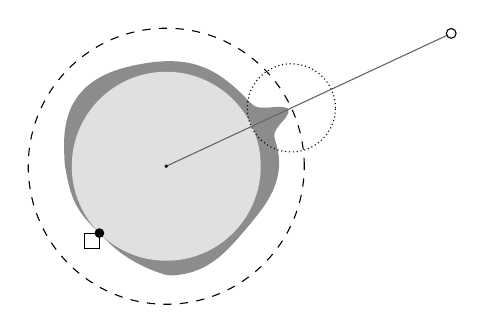
\begin{tikzpicture}[scale=0.8]
\fill[black!45] plot[smooth cycle,tension=0.6] coordinates {(1.790,0.000) (1.792,0.078) (1.787,0.156) (1.775,0.234) (1.759,0.310) (1.737,0.385) (1.718,0.460) (1.725,0.544) (1.795,0.653) (1.909,0.791) (1.941,0.905) (1.811,0.943) (1.612,0.931) (1.466,0.934) (1.383,0.968) (1.327,1.018) (1.276,1.070) (1.225,1.122) (1.173,1.173) (1.120,1.223) (1.066,1.271) (1.011,1.317) (0.954,1.362) (0.895,1.405) (0.835,1.446) (0.772,1.484) (0.708,1.519) (0.642,1.550) (0.574,1.578) (0.505,1.602) (0.435,1.623) (0.363,1.639) (0.291,1.652) (0.219,1.661) (0.146,1.666) (0.073,1.668) (0.000,1.668) (-0.073,1.664) (-0.145,1.659) (-0.217,1.651) (-0.289,1.641) (-0.361,1.630) (-0.433,1.617) (-0.505,1.603) (-0.577,1.586) (-0.650,1.568) (-0.722,1.548) (-0.794,1.525) (-0.865,1.499) (-0.936,1.469) (-1.006,1.437) (-1.074,1.400) (-1.140,1.359) (-1.203,1.313) (-1.264,1.264) (-1.320,1.209) (-1.372,1.151) (-1.419,1.089) (-1.462,1.023) (-1.499,0.955) (-1.530,0.884) (-1.557,0.810) (-1.578,0.736) (-1.595,0.660) (-1.607,0.585) (-1.615,0.509) (-1.620,0.434) (-1.622,0.360) (-1.622,0.286) (-1.620,0.213) (-1.617,0.141) (-1.614,0.070) (-1.607,0.000) (-1.594,-0.070) (-1.581,-0.138) (-1.567,-0.206) (-1.552,-0.274) (-1.535,-0.340) (-1.516,-0.406) (-1.493,-0.471) (-1.468,-0.534) (-1.439,-0.596) (-1.406,-0.656) (-1.370,-0.713) (-1.332,-0.769) (-1.291,-0.822) (-1.247,-0.873) (-1.202,-0.922) (-1.156,-0.970) (-1.108,-1.015) (-1.061,-1.061) (-1.015,-1.108) (-0.970,-1.156) (-0.923,-1.203) (-0.874,-1.249) (-0.824,-1.293) (-0.772,-1.336) (-0.717,-1.378) (-0.661,-1.418) (-0.603,-1.456) (-0.543,-1.493) (-0.482,-1.528) (-0.418,-1.561) (-0.353,-1.593) (-0.286,-1.624) (-0.218,-1.652) (-0.147,-1.679) (-0.074,-1.704) (-0.000,-1.726) (0.076,-1.733) (0.151,-1.729) (0.226,-1.720) (0.301,-1.707) (0.375,-1.689) (0.447,-1.667) (0.517,-1.640) (0.585,-1.609) (0.652,-1.573) (0.715,-1.534) (0.776,-1.491) (0.835,-1.446) (0.891,-1.398) (0.944,-1.349) (0.996,-1.298) (1.045,-1.246) (1.094,-1.193) (1.141,-1.141) (1.187,-1.088) (1.233,-1.034) (1.278,-0.981) (1.324,-0.927) (1.369,-0.872) (1.414,-0.816) (1.459,-0.760) (1.503,-0.701) (1.547,-0.641) (1.588,-0.578) (1.628,-0.513) (1.664,-0.446) (1.698,-0.376) (1.727,-0.304) (1.751,-0.231) (1.770,-0.155) (1.783,-0.078)};
\fill[black!12] (0,0) circle (1.500);
\draw[dashed] (0,0) circle (2.191);
\draw[densely dotted] (1.986,0.926) circle (0.700);
\draw[thin,black!60] (0,0) -- (4.524,2.109);
\filldraw[fill=white,draw=black] (-1.301,-1.301) rectangle (-1.061,-1.061);
\fill (-1.061,-1.061) circle (2.2pt);
\fill (0,0) circle (0.8pt);
\filldraw[fill=white,draw=black] (4.524,2.109) circle (2.2pt);
\end{tikzpicture}
\caption{The light disk is the largest ball $B(0,b)$ about the origin in~$D_n$, and the dark region is $E=D_n\setminus B(0,b)$. Every point of~$E$ contributes nonnegatively to~$U_E(y_0)$ at the contact point~$y_0$ (black dot), which lies on the circle $\{|v|=b\}$ and in the closure of a cell disjoint from~$D_n$ (square). The dashed circle, of radius $b+w=\Rout(n)+2\sqrt d$, contains~$D_n$, and the points of~$E$ in the dotted ball $B((b+w)u,t)$ contribute negatively to~$U_E(y_t)$ at the point $y_t=(b+w+4t)u$ (open dot) on the segment from the origin (small dot) in the direction of a unit vector~$u$.}
\label{fig:contact}
\end{figure}

Fix $p>0$. In this section and the next we take $n$ large and work on the event of Section~\ref{sec:norm-event}; its complement has probability at most $Cn^{-p}$, and on it $D_n\subset B(0,Kr_n)$, with $K$ as in Section~\ref{sec:norm-event}. Let $b\coloneqq\Rin(n)$ and $E\coloneqq D_n\setminus B(0,b)$, and let $y_0$ and~$H$ be as in Section~\ref{sec:largest-ball} for the Euclidean norm, so that $|y_0|=b$ and $H=U_{D_n}(y_0)=U_E(y_0)$.

If $s=|v|\geq b=|y_0|$, then
\begin{equation}\label{eq:contact-sign}
\frac{u_v\cdot(v-y_0)}{|v-y_0|^d}
=\frac{s^2-v\cdot y_0}{s|v-y_0|^d}
\geq\frac1{2s}|v-y_0|^{2-d}
\geq2^{1-d}s^{1-d}\, .
\end{equation}
The first inequality uses $2(s^2-v\cdot y_0)=|v-y_0|^2+s^2-b^2$, and the second $|v-y_0|\leq2s$ and $d\geq2$. Since $|v|\leq Cr_n$ on~$E$, integrating~\eqref{eq:contact-sign} over~$E$ gives $H\geq c|E|r_n^{1-d}$, and Lemma~\ref{lem:contact} gives
\begin{equation}\label{eq:mass}
|E|\leq Cr_n^{d-1}H\leq Cr_n^dq_n\, .
\end{equation}

\begin{proof}[Proof of Proposition~\ref{prop:inner}]
By~\eqref{eq:radius-volume} and~\eqref{eq:mass},
\begin{equation*}
\left|1-\left(\frac b{r_n}\right)^{d+1}\right|
\leq C\bigl(r_n^{\nf{(1-d)}{2}}(\log n)^{\nf12}+r_n^{-1}+q_n\bigr)
\leq Cq_n\, ,
\end{equation*}
because $r_n^{\nf{(1-d)}{2}}(\log n)^{\nf12}\leq q_n$. This proves~\eqref{eq:inradius}. Since $D_n$ is the disjoint union of~$B(0,b)$ and~$E$, the bounds~\eqref{eq:inradius} and~\eqref{eq:mass} prove~(ii).

On~$B(0,Kr_n)$, the bounds~\eqref{eq:norm-approx}, \eqref{eq:ballpotential-euclid}, \eqref{eq:potential-bound} and~\eqref{eq:inradius} give
\begin{equation*}
\bigl|\widetilde\ell_n(y)-2d\drift(r_n-|y|)_+\bigr|
\leq C\bigl(\sqrt{r_n}\log n+r_nq_n+|E|^{\nf1d}\bigr)\leq Cr_nq_n^{\nf1d}\, ,
\end{equation*}
and outside~$B(0,Kr_n)$ both $\widetilde\ell_n(y)$ and $2d\drift(r_n-|y|)_+$ vanish, which proves~(iii).
\end{proof}

\section{The outer radius and the local times}\label{sec:outer}

We prove the outer-radius and local-time bounds in Theorem~\ref{thm:fluctuations}. The crossing estimate~\eqref{eq:euclid-crossing} bounds the difference of the radii by $C\log n$ times one plus the largest local time outside the inner ball. To bound these local times, we bound the volume of the set~$E=D_n\setminus B(0,\Rin(n))$ near the outer sphere, the sphere about the origin of radius $\Rout(n)+2\sqrt d$. At a point beyond this sphere the potential is small, because the local time vanishes there. The points of~$E$ near that point contribute negatively to the potential, so a bound on the positive contributions bounds their volume (Figure~\ref{fig:contact}). Because the outer sphere is curved, the positive contributions are bounded by the integral of $|v-y|^{2-d}/|v|$ over~$E$. We first bound this integral by $Cr_nq_n$, using the volume bound in the plane and integrating the potential along rays in higher dimensions.

\begin{proposition}[Outer radius]\label{prop:stronger-outer}
Let $\gauge$ be the Euclidean norm, and let $0<\drift<\nf{1}{d}$. For every $p>0$ there exists $C(d,\drift,p)<\infty$ such that, for every integer~$n\geq2$, with probability at least $1-Cn^{-p}$,
\begin{equation*}
\Rout(n)\leq r_n+C\begin{cases}\sqrt{r_n}(\log n)^{\nf52},&d=2,\\(\log n)^{d+1},&d\geq3\end{cases}\, .
\end{equation*}
\end{proposition}

With $b=\Rin(n)$ and $E=D_n\setminus B(0,b)$, let
\begin{equation*}
w\coloneqq\Rout(n)-b+2\sqrt d
\qquad\text{and}\qquad
L\coloneqq1+\max\{\ell_n(x):x\in\Z^d,\ |x|\geq b\}\, .
\end{equation*}
Then $w\geq3\sqrt d/2\geq1$, because $b\leq\Rout(n)+\sqrt d/2$, and $E\subset\{b\leq|v|\leq b+w\}$. The outer-radius bound~\eqref{eq:norm-outer} for the Euclidean norm and~\eqref{eq:inradius} give
\begin{equation}\label{eq:width-preliminary}
w\leq Cr_nq_n^{\nf{1}{(d+1)}}\log n=o(r_n)\, ,
\end{equation}
so $1\leq w\leq b$ and $b\asymp r_n$ for large~$n$.
The crossing estimate~\eqref{eq:euclid-crossing} with $a=b$ gives $\Rout(n)\leq b+CL\log n$. Since $L\geq1$, this gives
\begin{equation}\label{eq:outer-width-occupation}
w\leq CL\log n\, .
\end{equation}

\subsection{The potential beyond the inner radius}\label{sec:outer-potential}

For a bounded measurable set~$D\subset\R^d$ and $y\in\R^d$, write
\begin{equation*}
U_D^+(y)\coloneqq\frac{2\drift}{\omega_d}\int_D\left[u_v\cdot\frac{v-y}{|v-y|^d}\right]_+\dd v
\end{equation*}
for the potential with its negative contributions discarded. If $|y|\geq b+w$, then every $v\in E$ satisfies $|v|\leq|y|$, so the identity $2(|v|^2-v\cdot y)=|v-y|^2+|v|^2-|y|^2$ gives $u_v\cdot(v-y)\leq|v-y|^2/(2|v|)$. Hence, with
\begin{equation*}
F(y)\coloneqq\int_E\frac{|v-y|^{2-d}}{|v|}\dd v\, ,
\end{equation*}
every $y\in\R^d$ with $|y|\geq b+w$ satisfies
\begin{equation}\label{eq:curvature-size}
U_E^+(y)\leq\frac\drift{\omega_d}F(y)\, .
\end{equation}
We prove that
\begin{equation}\label{eq:curvature-improved}
\sup_{\R^d}F\leq Cr_nq_n\, .
\end{equation}

\begin{proof}[Proof of~\eqref{eq:curvature-improved}]
If $d=2$, then $F(y)=\int_E|v|^{-1}\dd v\leq|E|/b$, so~\eqref{eq:mass} and $b\asymp r_n$ give the bound.

Suppose that $d\geq3$, and let $u$ be a unit vector. The derivative of $t^{d-2}|v-tu|^{2-d}$ in~$t>0$ is $(d-2)t^{d-3}v\cdot(v-tu)|v-tu|^{-d}$, so the definition of~$U_E$ gives
\begin{equation*}
\frac{\dd}{\dd t}\bigl(t^{d-2}F(tu)\bigr)=\frac{(d-2)\omega_d}{2\drift}t^{d-3}U_E(tu)\, .
\end{equation*}
For $t\geq b$ the ball potential vanishes, so~\eqref{eq:square-one-sided} gives $U_E(tu)=U_{D_n}(tu)\geq-Cr_nq_n$. Also $|v-2(b+w)u|\geq b+w$ and $|v|\geq b$ for $v\in E$, so~\eqref{eq:mass} gives $F(2(b+w)u)\leq|E|(b+w)^{2-d}/b\leq Cr_nq_n$. Integrating from~$t$ to~$2(b+w)$ gives, for $b\leq t\leq2(b+w)$,
\begin{equation*}
t^{d-2}F(tu)\leq\bigl(2(b+w)\bigr)^{d-2}F\bigl(2(b+w)u\bigr)+Cr_nq_n\int_t^{2(b+w)}s^{d-3}\dd s\leq Cr_n^{d-1}q_n\, .
\end{equation*}
Since $t\geq b\geq cr_n$, this proves the bound on $b\leq|y|\leq2(b+w)$. The function~$F$ is continuous, harmonic off the closure of~$E$, and tends to zero at infinity. The maximum principle extends the bound to~$B(0,b)$ and to the complement of~$B(0,2(b+w))$.
\end{proof}

\subsection{The volume near the outer sphere and the outer radius}

The following deterministic lemma bounds the positive contributions to the potential at a point between the two radii in terms of the volume near the sphere of radius~$b+w$.

\begin{lemma}\label{lem:near-far}
There exists $C(d,\drift)<\infty$ with the following property. Let $1\leq w\leq b$ and $\lambda\geq1$, and let $D$ be a measurable subset of $\{v\in\R^d:b\leq|v|\leq b+w\}$ such that $|D\cap B((b+w)u,t)|\leq\lambda t^{d-1}$ for every unit vector~$u$ and every $t\geq w$, and $\int_D|v-y|^{2-d}\dd v\leq\lambda b$ for every $y\in\R^d$. Then every $y\in\R^d$ with $b\leq|y|\leq b+w$ satisfies
\begin{equation*}
U_D^+(y)\leq C\bigl(\lambda w^{d-1}\bigr)^{\nf1d}+C\lambda\, .
\end{equation*}
\end{lemma}

\begin{proof}
Fix $y$ with $b\leq|y|\leq b+w$. If $t\geq w$, then $B(y,t)\subset B((b+w)u_y,2t)$, so $|D\cap B(y,t)|\leq2^{d-1}\lambda t^{d-1}$. In particular, the points of~$D$ within distance~$w$ of~$y$ have total volume at most $2^{d-1}\lambda w^{d-1}$, so, as in the proof of~\eqref{eq:potential-bound}, the integral of $|v-y|^{1-d}$ over them is at most $C(\lambda w^{d-1})^{\nf1d}$. For the other points~$v\in D$, both $|v|$ and~$|y|$ lie in~$[b,b+w]$, so the identity $2(|v|^2-v\cdot y)=|v-y|^2+|v|^2-|y|^2$ and $|v|^2-|y|^2\leq3bw$ give
\begin{equation*}
\left[u_v\cdot\frac{v-y}{|v-y|^d}\right]_+\leq\frac{2w}{|v-y|^d}+\frac1{2b|v-y|^{d-2}}\, .
\end{equation*}
The second term contributes at most $C\lambda$ to~$U_D^+(y)$, by the second hypothesis, and integrating the first by parts against the bound on $|D\cap B(y,t)|$ shows that it contributes at most $Cw\int_w^\infty\lambda t^{d-1}t^{-d-1}\dd t\leq C\lambda$.
\end{proof}

\begin{proof}[Proof of Proposition~\ref{prop:stronger-outer}]
\emph{Step 1: The volume of~$E$ near the sphere of radius~$b+w$.} We show that, for every unit vector~$u$ and every $t\geq w$,
\begin{equation}\label{eq:outer-cap-mass}
|E\cap B((b+w)u,t)|\leq Cr_nq_n t^{d-1}\, .
\end{equation}
For $t>\nf{r_n}4$ this follows from~\eqref{eq:mass}. So let $w\leq t\leq\nf{r_n}4$, and let $y_t\coloneqq(b+w+4t)u$ (Figure~\ref{fig:contact}). Every point of~$D_n$ lies within distance $\sqrt d/2$ of a site~$x$ with $|x|\leq\Rout(n)=b+w-2\sqrt d$, so $y_t\notin D_n$; also $U_{B(0,b)}(y_t)=0$. Thus~\eqref{eq:square-one-sided} gives $|U_E(y_t)|\leq Cr_nq_n$. If $v\in E\cap B((b+w)u,t)$, then $u_v\cdot u\geq1-t/(b+w)$, hence
\begin{equation*}
u_v\cdot(v-y_t)=|v|-(b+w+4t)u_v\cdot u\leq(b+w)-(b+w+4t)\left(1-\frac t{b+w}\right)\leq-t\, ,
\end{equation*}
where the last inequality uses $t\leq\nf{r_n}4\leq(b+w)/2$, which holds for large~$n$ by~\eqref{eq:inradius}. Since also $|v-y_t|\leq5t$, the kernel $u_v\cdot(v-y_t)|v-y_t|^{-d}$ is at most $-ct^{1-d}$ at each such~$v$. We bound $U_E(y_t)$ by the contributions of these points and the positive contributions of the remaining points of~$E$; by~\eqref{eq:curvature-size} and~\eqref{eq:curvature-improved},
\begin{equation*}
-Cr_nq_n\leq U_E(y_t)\leq Cr_nq_n-ct^{1-d}|E\cap B((b+w)u,t)|\, ,
\end{equation*}
which proves~\eqref{eq:outer-cap-mass}.

\emph{Step 2: The local times and the width.} Since $|v|\leq b+w\leq2b$ on~$E$, the bound~\eqref{eq:curvature-improved} gives $\int_E|v-y|^{2-d}\dd v\leq2bF(y)\leq Cbr_nq_n$ for every~$y$. Together with~\eqref{eq:outer-cap-mass}, this verifies the hypotheses of Lemma~\ref{lem:near-far} for $D=E$ and $\lambda=Cr_nq_n\geq1$. Thus, for $b\leq|y|\leq b+w$,
\begin{equation}\label{eq:positive-bound}
U_E^+(y)\leq C\bigl(r_nq_n w^{d-1}\bigr)^{\nf1d}+Cr_nq_n\, .
\end{equation}
For $|y|\geq b$, the ball potential vanishes, so~\eqref{eq:square-one-sided} gives
\begin{equation}\label{eq:envelopehigh}
\widetilde\ell_n(y)\leq2U_E(y)+Cr_nq_n\leq2U_E^+(y)+Cr_nq_n\, .
\end{equation}
Every site of~$A_n$ outside $B(0,b)$ lies in $b\leq|x|\leq b+w$, so~\eqref{eq:envelopehigh} and~\eqref{eq:positive-bound} give $L\leq C((r_nq_nw^{d-1})^{\nf1d}+r_nq_n)$. With~\eqref{eq:outer-width-occupation} and Young's inequality, this gives
\begin{equation*}
w\leq C\log n\Bigl(\bigl(r_nq_n w^{d-1}\bigr)^{\nf1d}+r_nq_n\Bigr)\leq\frac w2+Cr_nq_n(\log n)^d\, .
\end{equation*}
Consequently,
\begin{equation}\label{eq:outer-reduction}
w\leq Cr_nq_n(\log n)^d=C\begin{cases}\sqrt{r_n}(\log n)^{\nf52},&d=2,\\(\log n)^{d+1},&d\geq3\end{cases}\, .
\end{equation}
Since $\Rout(n)\leq b+w$ and $|b-r_n|\leq Cr_nq_n$ by~\eqref{eq:inradius}, this proves the proposition.
\end{proof}

\subsection{The uniform bound on the local times}\label{sec:global-profile}

We prove Theorem~\ref{thm:fluctuations}\,(iii) on the event of Section~\ref{sec:norm-event}, by bounding~$U_E$ on the annulus $\{b\leq|y|\leq b+w\}$, which contains~$E$. There the ball potential vanishes, so~\eqref{eq:square-one-sided} gives $U_E=U_{D_n}\geq-Cr_nq_n$, and $U_E\leq U_E^+$ and~\eqref{eq:positive-bound} give the upper bound. The function~$U_E$ is continuous, harmonic off the closure of~$E$, and tends to zero at infinity, so the maximum principle extends both bounds to $B(0,b)$ and to the complement of $B(0,b+w)$. With~\eqref{eq:outer-reduction}, this gives
\begin{equation*}
\sup_{\R^d}|U_E|\leq C\bigl((r_nq_n w^{d-1})^{\nf1d}+r_nq_n\bigr)
\leq Cr_nq_n(\log n)^{d-1}
=C\begin{cases}\sqrt{r_n}(\log n)^{\nf32},&d=2,\\(\log n)^d,&d\geq3\end{cases}\, .
\end{equation*}
On $B(0,Kr_n)$, combine this with~\eqref{eq:norm-approx}, $U_{D_n}(y)=2d\drift(b-|y|)_++U_E(y)$ and $|b-r_n|\leq Cr_nq_n$ to obtain the claimed bound. Outside this ball both the local time and $2d\drift(r_n-|y|)_+$ vanish.

\begin{proof}[Proof of Theorem~\ref{thm:fluctuations}]
On the event of Section~\ref{sec:norm-event}, for large~$n$, Proposition~\ref{prop:inner} gives the bounds on~$\Rin(n)$ and on the volume, Proposition~\ref{prop:stronger-outer} the bound on~$\Rout(n)$, and Section~\ref{sec:global-profile} the bound on the local times. The Borel--Cantelli lemma with $p>1$ gives the almost-sure statement.
\end{proof}

\section{Limit laws}\label{sec:sharp}

We prove central limit theorems and laws of the iterated logarithm for $\sum_{x\in A_n}|x|$ and for the local times at fixed sites. After centering, these quantities are, up to smaller errors, linear combinations of the martingale~$\mathcal Q$ of~\eqref{eq:quadratic} and of the martingales~$\mathcal M^y$ of Section~\ref{sec:dynkin}; we compute the limits of their brackets from Theorem~\ref{thm:shape}\,(ii), and then apply the martingale central limit theorem and the law of the iterated logarithm.

We use these two theorems in the following form, here and in Section~\ref{sec:lower}. Let $Z$ be a real square-integrable martingale with $Z_0=0$, and let $s_n\to\infty$ be deterministic with $\log\log s_n\sim\log\log n$. Suppose that $\langle Z\rangle_n/s_n^2\to\sigma^2$ almost surely for a constant $\sigma\geq0$ and that $|Z_{j+1}-Z_j|\leq\eta_j$ for $\mathcal F_j$-measurable~$\eta_j$ with $\max_{j<n}\eta_j=o(s_n(\log\log n)^{-\nf12})$ almost surely. Then $Z_n/s_n$ converges in distribution to $\mathcal N(0,\sigma^2)$ \citep[Corollary~3.1]{HallHeyde1980}, and, if $\sigma>0$, then $\limsup_{n\to\infty}\pm Z_n/(s_n\sqrt{2\log\log n})=\sigma$ almost surely for each sign \citep[Theorems~1 and~2]{Stout1970}. For a vector martingale satisfying these hypotheses in every direction with the same~$s_n$, the Cram\'er--Wold device gives a joint Gaussian limit.

\subsection{The sum of the distances from the origin}

For the Euclidean norm, \eqref{eq:quadratic} reads
\begin{equation}\label{eq:moment-martingale}
\mathcal Q_n=2\drift\sum_{x\in A_n}|x|-n+|X_n|^2\, .
\end{equation}
Let $\Rmom(n)$ be the radius of the ball about the origin on which the integral of~$|v|$ equals $\sum_{x\in A_n}|x|$, that is,
\begin{equation}\label{eq:radial-moment-def}
\Rmom(n)\coloneqq\left(\frac{d+1}{d\omega_d}\sum_{x\in A_n}|x|\right)^{\nf{1}{(d+1)}}\, .
\end{equation}

\begin{theorem}[Sum of the distances from the origin]\label{thm:moment-fluctuations}
Let $\gauge$ be the Euclidean norm, let $0<\drift<\nf1d$, and let $\Rmom(n)$ be as in~\eqref{eq:radial-moment-def}. Then the following hold.
\begin{enumerate}[label=\textup{(\roman*)}]
\item \underline{\emph{Central limit theorem}}: as $n\to\infty$,
\begin{equation*}
\frac{\sum_{x\in A_n}|x|-n/(2\drift)}{r_n^{\nf{(d+3)}{2}}}
\xrightarrow{\mathrm d}\mathcal N\Bigl(0,\frac{2d\omega_d}{\drift(d+2)(d+3)}\Bigr)
\end{equation*}
and
\begin{equation*}
\frac{\Rmom(n)-r_n}{r_n^{\nf{(3-d)}{2}}}
\xrightarrow{\mathrm d}\mathcal N\Bigl(0,\frac{2}{\drift d\omega_d(d+2)(d+3)}\Bigr)\, .
\end{equation*}
\item \underline{\emph{Law of the iterated logarithm}}: for each choice of sign, almost surely,
\begin{align}
\limsup_{n\to\infty}\frac{\pm\bigl(\sum_{x\in A_n}|x|-n/(2\drift)\bigr)}{r_n^{\nf{(d+3)}{2}}\sqrt{2\log\log n}}
&=\Bigl(\frac{2d\omega_d}{\drift(d+2)(d+3)}\Bigr)^{\nf12}\, ,\notag\\
\limsup_{n\to\infty}\frac{\pm(\Rmom(n)-r_n)}{r_n^{\nf{(3-d)}{2}}\sqrt{2\log\log n}}
&=\Bigl(\frac{2}{\drift d\omega_d(d+2)(d+3)}\Bigr)^{\nf12}\, .\label{eq:moment-radius-lil}
\end{align}
\end{enumerate}
\end{theorem}

In the plane, comparing $\Rmom(n)$ with the inner and outer radii gives Theorem~\ref{thm:sharp}\,(ii) and, with a lower bound on the probability that~$\mathcal Q_n$ deviates by about $(\log n)^{\nf12}$ standard deviations (Lemma~\ref{lem:exp-deviation}), Theorem~\ref{thm:sharp}\,(i).

\begin{proof}[Proof of Theorem~\ref{thm:moment-fluctuations}]
\emph{Step 1: The bracket.} Under both~\eqref{eq:kernel} and the simple random walk transition probabilities, the conditional second-moment matrix of $X_{j+1}-X_j$ is $d^{-1}$ times the identity. Thus, for an $\mathcal F_j$-measurable vector~$q$, the conditional variance of $q\cdot(X_{j+1}-X_j)$ is $|q|^2/d-\drift^2I_j(q\cdot u_{X_j})^2$. Since $\mathcal Q_{j+1}-\mathcal Q_j=2X_j\cdot(X_{j+1}-X_j+\drift I_ju_{X_j})$, this gives
\begin{equation}\label{eq:moment-exact-bracket}
\langle\mathcal Q\rangle_n=\frac4d\sum_{x\in\Z^d}\ell_n(x)|x|^2-4\drift^2\sum_{x\in A_n}|x|^2\, .
\end{equation}
Theorem~\ref{thm:shape} gives $\Rout(n)=O(r_n)$ and uniform convergence of the rescaled local times to $2d\drift(1-|v|)_+$ almost surely. Hence the first sum, divided by $r_n^{d+3}$, converges to
\begin{equation*}
2d\drift\int_{|v|<1}(1-|v|)|v|^2\dd v=\frac{2d^2\drift\omega_d}{(d+2)(d+3)}\, .
\end{equation*}
The second sum is $O(r_n^{d+2})$, so
\begin{equation}\label{eq:moment-bracket-limit}
\frac{\langle\mathcal Q\rangle_n}{r_n^{d+3}}\longrightarrow\frac{8d\drift\omega_d}{(d+2)(d+3)}
\qquad\text{almost surely}\, .
\end{equation}

\emph{Step 2: The limit laws.} Since $|\mathcal Q_{j+1}-\mathcal Q_j|\leq4|X_j|$ and $\Rout(n)=O(r_n)$ almost surely, the limit theorems stated at the beginning of this section apply to~$\mathcal Q$ with $s_n=r_n^{\nf{(d+3)}2}$ and the variance~\eqref{eq:moment-bracket-limit}. In~\eqref{eq:moment-martingale}, the endpoint term $|X_n|^2=O(r_n^2)$ is negligible on both scales, giving the assertions for the sum. These also give $\Rmom(n)/r_n\to1$ almost surely. Expanding~\eqref{eq:radial-moment-def} now gives
\begin{equation*}
\frac{\Rmom(n)-r_n}{r_n^{\nf{(3-d)}2}}
=\left(\frac1{d\omega_d}+o(1)\right)
\frac{\sum_{x\in A_n}|x|-n/(2\drift)}{r_n^{\nf{(d+3)}2}}\, ,
\end{equation*}
which gives both assertions for~$\Rmom(n)$.
\end{proof}

\subsection{The potential at a fixed site}

Since $B(0,\Rin(n))\subset D_n\subset B(0,\Rout(n)+\sqrt d)$, Theorem~\ref{thm:fluctuations}\,(i) and~(ii) give, almost surely for all large~$n$, $|D_n\mathbin{\triangle}B(0,r_n)|\leq Cr_n^dq_n$ and, for every $v\in D_n\mathbin{\triangle}B(0,r_n)$,
\begin{equation}\label{eq:centering-shape-input}
\bigl||v|-r_n\bigr|\leq C\begin{cases}\sqrt{r_n}(\log n)^{\nf52},&d=2,\\(\log n)^{d+1},&d\geq3\end{cases}\, .
\end{equation}
For a fixed site~$y$, on the annulus defined by~\eqref{eq:centering-shape-input} the kernel of~$U_{D_n}(y)$ is close to $r_n^{-d}|v|$, which relates $U_{D_n}(y)$ to $\sum_{x\in A_n}|x|$ and hence, by~\eqref{eq:moment-martingale}, to~$\mathcal Q_n$.

\begin{lemma}\label{lem:fixed-site-centering}
Let $\gauge$ be the Euclidean norm, let $0<\drift<\nf1d$, and let $y\in\Z^d$. There exists $C(d,\drift,y)<\infty$ such that, almost surely, for all sufficiently large~$n$,
\begin{equation}\label{eq:fixed-site-centering}
\left|U_{D_n}(y)-2d\drift(r_n-|y|)-\frac{\mathcal Q_n}{\omega_dr_n^d}\right|\leq C\begin{cases}(\log n)^3,&d=2,\\1,&d\geq3\end{cases}\, ,
\end{equation}
where $\mathcal Q$ is the martingale of~\eqref{eq:quadratic}.
\end{lemma}

By Theorem~\ref{thm:moment-fluctuations}, $\mathcal Q_n/(\omega_dr_n^d)$ has order~$r_n^{\nf{(3-d)}{2}}$, smaller than the order of~$\mathcal M^y_n$ by a factor~$(\log r_n)^{\nf12}$ in the plane and~$r_n^{\nf{(d-2)}{2}}$ when $d\geq3$.

\begin{proof}
Write $r=r_n$, $\nu=\ind_{D_n}-\ind_{B(0,r)}$, and $w=\sup_{v\in\operatorname{supp}\nu}\bigl||v|-r\bigr|$. By~\eqref{eq:centering-shape-input}, $w=o(r)$ and $\|\nu\|_1\leq Cr^dq_n$. For fixed~$y$ and $v\in\operatorname{supp}\nu$, Taylor's formula gives
\begin{equation*}
\frac{v}{|v|}\cdot\frac{v-y}{|v-y|^d}
=|v|^{1-d}+O_y(r^{-d})
=r^{-d}|v|+O_y\bigl(r^{-d}(1+w)\bigr)\, .
\end{equation*}
Integrating against~$\nu$ and using~\eqref{eq:ballpotential-euclid} therefore gives
\begin{equation*}
U_{D_n}(y)-2d\drift(r-|y|)
=\frac{2\drift}{\omega_dr^d}
\left(\int_{D_n}|v|\dd v-\frac n{2\drift}\right)
+O_y\bigl(q_n(1+w)\bigr)\, .
\end{equation*}
Replacing the integral by $\sum_{x\in A_n}|x|$ costs $O(r^d)$. By~\eqref{eq:moment-martingale}, the main term is thus $\mathcal Q_n/(\omega_dr^d)+O(1)$, since $|X_n|^2/r^d=O(1)$. Finally, \eqref{eq:centering-shape-input} gives $q_n(1+w)=O((\log n)^3)$ in the plane and $O((\log n)^{d+2}/r)=O(1)$ in higher dimensions.
\end{proof}

\subsection{Local times at fixed sites}

Up to a smaller correction at first departures, the bracket of~$\mathcal M^y$ is a sum of local times with weights that decay like~$|x-y|^{2-2d}$; in the plane each dyadic annulus about~$y$ inside~$B(0,r_n)$ contributes order~$r_n$, which gives an extra factor~$\log r_n$. For functions $f_1,f_2\colon\Z^d\to\R$ with bounded nearest-neighbor increments, let
\begin{equation}\label{eq:site-gamma}
\Gamma(f_1,f_2)(x)\coloneqq\frac1{2d}\sum_{|e|=1}\bigl(f_1(x+e)-f_1(x)\bigr)\bigl(f_2(x+e)-f_2(x)\bigr)-\Delta f_1(x)\Delta f_2(x)\, ,
\end{equation}
which is the conditional covariance of the increments of~$\mathcal M^{f_1}$ and~$\mathcal M^{f_2}$ at a departure from~$x$ other than the first. As in Section~\ref{sec:dynkin}, $g_y=g(\cdot-y)$ and $G$ is the Green function.

\begin{theorem}[Local times at fixed sites]\label{thm:site-fluctuations}
Let $\gauge$ be the Euclidean norm, and let $0<\drift<\nf1d$. Then the following hold.
\begin{enumerate}[label=\textup{(\roman*)}]
\item \underline{\emph{Central limit theorem}}: for every $y\in\Z^d$, as $n\to\infty$,
\begin{equation}\label{eq:site-clt}
\begin{aligned}
\frac{\ell_n(y)-2d\drift(r_n-|y|)}{\sqrt{r_n\log r_n}}&\xrightarrow{\mathrm d}\mathcal N\Bigl(0,\frac{16\drift}{\pi}\Bigr)&&\text{if } d=2\, ,\\
\frac{\ell_n(y)-2d\drift(r_n-|y|)}{\sqrt{r_n}}&\xrightarrow{\mathrm d}\mathcal N\bigl(0,2d\drift(2G(0)-1)\bigr)&&\text{if } d\geq3\, .
\end{aligned}
\end{equation}
\item \underline{\emph{Law of the iterated logarithm}}: for every $y\in\Z^d$ and each choice of sign, almost surely,
\begin{equation*}
\begin{aligned}
\limsup_{n\to\infty}\frac{\pm(\ell_n(y)-2d\drift(r_n-|y|))}{\sqrt{2r_n\log r_n\log\log n}}&=\Bigl(\frac{16\drift}{\pi}\Bigr)^{\nf12}&&\text{if } d=2\, ,\\
\limsup_{n\to\infty}\frac{\pm(\ell_n(y)-2d\drift(r_n-|y|))}{\sqrt{2r_n\log\log n}}&=\bigl(2d\drift(2G(0)-1)\bigr)^{\nf12}&&\text{if } d\geq3\, .
\end{aligned}
\end{equation*}
\item \underline{\emph{Joint limits}}: for all $y_1,\ldots,y_k\in\Z^d$, the convergence in~\eqref{eq:site-clt} holds jointly for $y=y_1,\ldots,y_k$, and the limit is a centered Gaussian vector whose covariance matrix has $(i,j)$ entry
\begin{equation}\label{eq:site-covariance}
\begin{cases}
16\drift/\pi,&d=2,\\
2d\drift\bigl(2G(y_i-y_j)-\ind_{\{y_i=y_j\}}\bigr),&d\geq3
\end{cases}\, .
\end{equation}
\end{enumerate}
\end{theorem}

In the plane the limits at different sites are equal; this statement concerns finitely many fixed sites, whereas the maximum in Theorem~\ref{thm:sharp}\,(iii) is over the sites~$x$ with $|x|\leq r_n^{\nf12}$, a set that grows with~$n$.

\begin{proof}[Proof of Theorem~\ref{thm:site-fluctuations}]
\emph{Step 1: The bracket.} A first departure from~$x$ changes the conditional covariance from $\Gamma(g_y,g_z)(x)$ by $O_{y,z}((1+|x|)^{2-2d})$, by~\eqref{eq:gradient}. There is one such departure per site of~$A_n$, which is contained in $B(0,Cr_n)$ eventually almost surely. Thus
\begin{equation}\label{eq:site-bracket}
\langle\mathcal M^y,\mathcal M^z\rangle_n
=\sum_{x\in\Z^d}\ell_n(x)\Gamma(g_y,g_z)(x)
+\begin{cases}O_{y,z}(\log r_n),&d=2,\\O_{y,z}(1),&d\geq3\end{cases}\, .
\end{equation}

\emph{Step 2: The bracket in higher dimensions.} The identity $\Gamma(f,h)=\Delta(fh)-f\Delta h-h\Delta f-\Delta f\Delta h$ gives
\begin{equation*}
\sum_x\Gamma(f,h)(x)=-\sum_x\bigl(f(x)\Delta h(x)+h(x)\Delta f(x)+\Delta f(x)\Delta h(x)\bigr)
\end{equation*}
whenever the boundary term vanishes. For $f=g_y$ and $h=g_z$ in $d\geq3$ it is $O(R^{2-d})$ on a ball of radius~$R$, by~\eqref{eq:kernel-asymptotics} and~\eqref{eq:gradient}. Since $\Delta g_y=\ind_{\{y\}}$, the sum is $2G(y-z)-\ind_{\{y=z\}}$. The weights are absolutely summable, so Theorem~\ref{thm:shape}\,(ii) and dominated convergence give
\begin{equation*}
\frac{\langle\mathcal M^y,\mathcal M^z\rangle_n}{r_n}
\longrightarrow2d\drift\bigl(2G(y-z)-\ind_{\{y=z\}}\bigr)
\qquad\text{almost surely}\, .
\end{equation*}

\emph{Step 3: The bracket in the plane.} The asymptotic formulas~\eqref{eq:kernel-asymptotics} and~\eqref{eq:gradient} give, for fixed~$y,z$,
\begin{equation*}
\Gamma(g_y,g_z)(x)=\frac2{\pi^2|x|^2}+O_{y,z}(|x|^{-3}),
\qquad
\sum_{|x|\leq r}\Gamma(g_y,g_z)(x)=\frac4\pi\log r+O_{y,z}(1)\, .
\end{equation*}
In~\eqref{eq:site-bracket}, the uniform error $o(r_n)$ of Theorem~\ref{thm:shape}\,(ii) costs $o(r_n\log r_n)$. The term $4\drift r_n$ contributes $(16\drift/\pi)r_n\log r_n+O(r_n)$. The term $-4\drift|x|$ contributes $O(r_n)$, since
\begin{equation*}
\sum_{|x|\leq r_n}|x|\,|\Gamma(g_y,g_z)(x)|=O(r_n)\, .
\end{equation*}
Therefore
\begin{equation*}
\frac{\langle\mathcal M^y,\mathcal M^z\rangle_n}{r_n\log r_n}
\longrightarrow\frac{16\drift}{\pi}
\qquad\text{almost surely}\, .
\end{equation*}

\emph{Step 4: The limit laws.} The martingales~$\mathcal M^y$ have bounded increments, so by Steps~2 and~3 the limit theorems stated at the beginning of this section apply to the vector $(-\mathcal M^{y_i})_{i\leq k}$, with $s_n=\sqrt{r_n\log r_n}$ if $d=2$ and $s_n=\sqrt{r_n}$ if $d\geq3$. Finally~\eqref{eq:pointwise} and Lemma~\ref{lem:fixed-site-centering} give
\begin{equation*}
\ell_n(y)-2d\drift(r_n-|y|)
=-\mathcal M_n^y+\frac{\mathcal Q_n}{\omega_dr_n^d}
+\begin{cases}O_y((\log n)^3),&d=2,\\O_y(\log n),&d\geq3\end{cases}\, .
\end{equation*}
Theorem~\ref{thm:moment-fluctuations} makes the last two terms negligible on both normalizations, proving all three assertions.
\end{proof}

\section{Lower bounds on the fluctuations}\label{sec:lower}

We prove the lower bounds of Theorem~\ref{thm:sharp}, an upper bound on the deviations of the local times away from the boundary (Proposition~\ref{prop:bulk-profile}), and logarithmic lower bounds on the radii (Proposition~\ref{prop:log-lower}). The lower bounds in Theorem~\ref{thm:sharp}\,(i), (iii) and~(iv)(a) need martingale deviations of about $(\log n)^{\nf12}$ standard deviations. We obtain them from exponential martingales (Lemma~\ref{lem:exp-deviation}): for parts~(i) and~(iv)(a) by the Paley--Zygmund inequality for one exponential martingale, and for part~(iii) by a second-moment bound for the average of the exponential martingales at many well-separated sites. Part~(iii) needs many sites because, by Theorem~\ref{thm:site-fluctuations}, the deviation at one fixed site is typically smaller than the bound in part~(iii) by a factor of order~$(\log n)^{\nf12}$.

Throughout this section $0<\drift<\nf1d$, and $\Omega_n$ is the event of Section~\ref{sec:norm-event} with $p=10$, so $\P(\Omega_n^c)=O(n^{-10})$ and the estimates of Sections~\ref{sec:local}--\ref{sec:outer} used below hold on~$\Omega_n$ for large~$n$. In particular, by Section~\ref{sec:global-profile}, on~$\Omega_n$ for large~$n$, in every dimension,
\begin{equation}\label{eq:lower-local-error}
\max_{x\in\Z^d}\bigl|\ell_n(x)-2d\drift(r_n-|x|)_+\bigr|\leq C\sqrt{r_n}(\log n)^{\nf32}\, .
\end{equation}

\begin{lemma}\label{lem:exp-deviation}
Let $0<c_0\leq C_0$. There exist $c(c_0,C_0)>0$ and $C(c_0,C_0)<\infty$ with the following property. Let $m$ and~$n$ be positive integers, let $b>0$, $\delta\geq0$ and $0\leq\alpha\leq1$, and let $S^1,\ldots,S^m$ be real martingales with respect to a common filtration, with $S^i_0=0$ and $|S^i_{t+1}-S^i_t|\leq b$ for $0\leq t<n$. Let $\Omega$ be an event with $\P(\Omega)\geq1-\alpha$ on which $c_0\leq\langle S^i\rangle_n\leq C_0$ for $1\leq i\leq m$. Then, for every real $\beta\geq C$ with $\beta b\leq c$, the following hold.
\begin{enumerate}[label=\textup{(\roman*)}]
\item For $1\leq i\leq m$,
\begin{equation*}
\P(S^i_n\geq c\beta)\geq\frac14e^{-C\beta^2}-\alpha
\qquad\text{and}\qquad
\P(S^i_n\leq-c\beta)\geq\frac14e^{-C\beta^2}-\alpha\, .
\end{equation*}
\item If $|\langle S^i,S^j\rangle_n|\leq\delta$ on~$\Omega$ for all $i\neq j$, and $\beta^2\delta+\beta^3b\leq1$, then
\begin{equation*}
\P\Bigl(\max_{1\leq i\leq m}S^i_n<c\beta\Bigr)\leq C\bigl(m^{-1}e^{C\beta^2}+\beta^2\delta+\beta^3b+e^{C\beta^2}\sqrt\alpha\bigr)\, .
\end{equation*}
\end{enumerate}
\end{lemma}

\begin{proof}
Let $(\mathcal G_t)_{0\leq t\leq n}$ be the filtration, let $\tau$ be the least integer $0\leq t<n$ such that $\langle S^i\rangle_{t+1}>2C_0$ for some~$i$, and let $\tau=n$ if there is none. Since brackets are predictable, $\tau$ is a stopping time. On~$\Omega$ we have $\tau=n$, so replacing each $S^i$ by $S^i$ stopped at~$\tau$ changes neither the hypotheses nor~$S^i_n$ on~$\Omega$, and gives $\langle S^i\rangle_n\leq2C_0$. Let $V_{ij}=\langle S^i,S^j\rangle_n$, so that $|V_{ij}|\leq2C_0$ by the Cauchy--Schwarz inequality. We take $c\leq\min\{\nf14,\nf{c_0}8\}$ small and $C$ large, both depending only on $c_0$ and~$C_0$.

Let $S$ be a martingale with respect to~$(\mathcal G_t)$, with $S_0=0$, increments of absolute value at most~$b_1$ and $\langle S\rangle_n\leq8C_0$, let $|s|b_1\leq\nf12$, and let
\begin{equation*}
\psi(s)\coloneqq\sum_{t<n}\log\E\bigl(e^{s(S_{t+1}-S_t)}\bigm|\mathcal G_t\bigr)
\qquad\text{and}\qquad
W(s)\coloneqq\exp\{sS_n-\psi(s)\}\, .
\end{equation*}
By successive conditioning $\E W(s)=1$. Since each increment $S_{t+1}-S_t$ has conditional mean zero and absolute value at most~$b_1$, Taylor's formula for the exponential and the logarithm gives, whenever $|s|b_1\leq1$ and with an absolute implicit constant,
\begin{equation}\label{eq:exp-taylor}
\log\E\bigl(e^{s(S_{t+1}-S_t)}\bigm|\mathcal G_t\bigr)=\frac{s^2}2\E\bigl((S_{t+1}-S_t)^2\bigm|\mathcal G_t\bigr)\bigl(1+O(|s|b_1)\bigr)\, .
\end{equation}
Summing~\eqref{eq:exp-taylor} over $t<n$ gives $\psi(s)=s^2\langle S\rangle_n/2+O(|s|^3b_1)$, and the same holds at~$2s$. Hence $\psi(2s)-2\psi(s)\leq Cs^2$, and since $W(s)^2=W(2s)\exp\{\psi(2s)-2\psi(s)\}$, we get $\E W(s)^2\leq e^{Cs^2}$. We apply these definitions and bounds with $s=\beta$ to~$S^i$, with $b_1=b$, and to $S^i+S^j$ for $i\neq j$, whose bracket at time~$n$ is $V_{ii}+V_{jj}+2V_{ij}\leq8C_0$, with $b_1=2b$; this is possible because $\beta b\leq\nf14$. Let $\psi_i$, $W_i$ and $\psi_{ij}$, $W_{ij}$ be the corresponding values of $\psi(\beta)$ and~$W(\beta)$. Then
\begin{equation}\label{eq:exp-moments}
\psi_i=\frac{\beta^2}2V_{ii}+O(\beta^3b)
\qquad\text{and}\qquad
\psi_{ij}-\psi_i-\psi_j=\beta^2V_{ij}+O(\beta^3b)\, ,
\end{equation}
and $\E W_i=\E W_{ij}=1$, $\E W_i^2\leq e^{C\beta^2}$ and $\E W_{ij}^2\leq e^{C\beta^2}$.

We prove~(i). If $c$ is small enough, then on~$\Omega$ the bound $V_{ii}\geq c_0$ and~\eqref{eq:exp-moments} give $\psi_i\geq c_0\beta^2/4$. If also $C$ is large enough, then on~$\Omega$ the inequality $W_i\geq\nf12$ implies $\beta S^i_n\geq c_0\beta^2/4-\log2$, hence $S^i_n\geq c_0\beta/8\geq c\beta$. By the Paley--Zygmund inequality, $\P(W_i\geq\nf12)\geq(\E W_i)^2/(4\E W_i^2)\geq e^{-C\beta^2}/4$, so $\P(S^i_n\geq c\beta)\geq\P(\Omega\cap\{W_i\geq\nf12\})\geq e^{-C\beta^2}/4-\alpha$. The same argument applied to~$-S^i$ gives the second bound in~(i).

We prove~(ii). Let $i\neq j$. By~\eqref{eq:exp-moments}, the exponent in $W_iW_j=W_{ij}\exp\{\psi_{ij}-\psi_i-\psi_j\}$ is at most $\beta^2\delta+C\beta^3b$ on~$\Omega$, and at most $C\beta^2$ everywhere, because $|V_{ij}|\leq2C_0$ and $\beta b\leq1$. So the Cauchy--Schwarz inequality on~$\Omega^c$ and $\beta^2\delta+\beta^3b\leq1$ give
\begin{equation*}
\E(W_iW_j)\leq e^{\beta^2\delta+C\beta^3b}+e^{C\beta^2}\bigl(\E W_{ij}^2\bigr)^{\nf12}\alpha^{\nf12}\leq1+C(\beta^2\delta+\beta^3b)+e^{C\beta^2}\sqrt\alpha\, .
\end{equation*}
Let $\overline W\coloneqq m^{-1}\sum_{i=1}^mW_i$. Then $\E\overline W=1$, and the bounds on $\E W_i^2$ and on $\E(W_iW_j)$ give
\begin{equation*}
\Var(\overline W)=\frac1{m^2}\sum_{i,j=1}^m\bigl(\E(W_iW_j)-1\bigr)\leq C\bigl(m^{-1}e^{C\beta^2}+\beta^2\delta+\beta^3b+e^{C\beta^2}\sqrt\alpha\bigr)\, .
\end{equation*}
On~$\Omega$, if $\overline W\geq\nf12$, then $W_i\geq\nf12$ for some~$i$, and hence $\max_iS^i_n\geq c\beta$, as in the proof of~(i). So Chebyshev's inequality gives $\P(\max_iS^i_n<c\beta)\leq4\Var(\overline W)+\alpha$, which proves~(ii), because $\alpha\leq\sqrt\alpha$.
\end{proof}

\subsection{Lower bounds on the radii and their difference in the plane}

Up to additive constants, $\Rin(n)\leq\Rmom(n)\leq\Rout(n)$, and by~\eqref{eq:moment-martingale} the difference $\Rmom(n)-r_n$ is, to first order, proportional to~$\mathcal Q_n$. So Theorem~\ref{thm:sharp}\,(i) needs deviations of~$\mathcal Q_n$ of about $(\log n)^{\nf12}$ standard deviations with probability at least~$n^{-p}$. Lemma~\ref{lem:exp-deviation}\,(i) gives them from the coarse bounds: the upper bound on each local time forces a positive fraction of the steps to occur at distance comparable to~$r_n$, which bounds the bracket of~$\mathcal Q$ below. For part~(iv) we use the martingale $Z_n=X_n+\drift\sum_{x\in A_n}u_x$ of~\eqref{eq:vector-def}. The vectors~$u_x$ cancel over the sites inside the inner disk, so $|Z_n-X_n|$ is at most $\drift(\Rout(n)^2-\Rin(n)^2)+Cr_n$ when both radii lie between $r_n/2$ and~$2r_n$. Lemma~\ref{lem:exp-deviation}\,(i) for the first coordinate of~$Z$, whose bracket lies between two constant multiples of~$n$ on every path, gives part~(iv)(a); the martingale law of the iterated logarithm for the same coordinate gives part~(iv)(b), and the martingale central limit theorem for~$Z$ gives part~(iv)(c).

\begin{proof}[Proof of Theorem~\ref{thm:sharp}\,\textup{(i)} and~\textup{(ii)}]
Comparison with unit cells gives $\sum_{|x|<r}|x|=d\omega_dr^{d+1}/(d+1)+O(r^d)$. Since every lattice site in $B(0,\Rin(n))$ belongs to~$A_n$ and $A_n\subset B(0,\Rout(n)+1)$, taking $(d+1)$st roots gives, for every path,
\begin{equation}\label{eq:moment-radius-comparison}
\Rin(n)\leq\Rmom(n)+C
\qquad\text{and}\qquad
\Rout(n)\geq\Rmom(n)-C\, .
\end{equation}
For $d=2$, the two signs in~\eqref{eq:moment-radius-lil} therefore give~\eqref{eq:planar-lil-lower}, with constant $\sqrt2/\sqrt{20\pi\drift}=1/\sqrt{10\pi\drift}$.

For the polynomial lower bounds, let $r=r_n$ and use the stopped martingale~$\widehat{\mathcal Q}$ from Section~\ref{sec:norm-event}. Its increments are at most $4Kr$, and it agrees with~$\mathcal Q$ through time~$n$ on~$\Omega_n$. The coarse bounds $\max_x\ell_n(x)\leq Cr$ and $\Rout(n)\leq Cr$, together with $\sum_x\ell_n(x)=n$, force at least $n/2$ departures to occur outside $B(0,cr)$ for a fixed sufficiently small $c>0$. Since $\drift<1/2$, the exact bracket~\eqref{eq:moment-exact-bracket} therefore gives fixed $0<c_0<C_0<\infty$ such that, for all large~$n$,
\begin{equation*}
c_0r^5\leq\langle\widehat{\mathcal Q}\rangle_n\leq C_0r^5
\qquad\text{on }\Omega_n\, .
\end{equation*}
Let $c_1,C_1$ be the constants of Lemma~\ref{lem:exp-deviation} for these bracket bounds, and choose $a_p>0$ with $C_1a_p^2\leq\min\{p,10\}/2$. Apply part~(i) of that lemma to $\widehat{\mathcal Q}/r^{\nf52}$, with $b=4Kr^{-\nf32}$, $\beta=a_p\sqrt{\log n}$ and $\alpha=\P(\Omega_n^c)=O(n^{-10})$. For all large~$n$, each of
\begin{equation*}
\{\mathcal Q_n\geq c_1a_pr^{\nf52}\sqrt{\log n}\}\cap\Omega_n
\quad\text{and}\quad
\{\mathcal Q_n\leq-c_1a_pr^{\nf52}\sqrt{\log n}\}\cap\Omega_n
\end{equation*}
has probability at least $n^{-\min\{p,10\}/2}/4-O(n^{-10})\geq n^{-p}$. On~$\Omega_n$, $|X_n|^2=O(r^2)$ and $\Rmom(n)=O(r)$. Consequently~\eqref{eq:moment-martingale} and
\begin{equation*}
\Rmom(n)^3-r^3=\frac3{2\pi}\left(\sum_{x\in A_n}|x|-\frac n{2\drift}\right)
\end{equation*}
show that the first event forces $\Rmom(n)-r\geq c\sqrt{r\log n}$, and the second forces $r-\Rmom(n)\geq c\sqrt{r\log n}$. Now~\eqref{eq:moment-radius-comparison} proves~\eqref{eq:planar-polynomial-lower}.
\end{proof}

\begin{proof}[Proof of Theorem~\ref{thm:sharp}\,\textup{(iv)}]
Let $d=2$, $V_n=\sum_{x\in A_n}u_x$, and $Z_n=X_n+\drift V_n$, the martingale of~\eqref{eq:vector-def}. Its increments are bounded by~$2$, and the conditional second-moment calculation in Step~1 of the proof of Theorem~\ref{thm:moment-fluctuations} gives, for every $q\in\R^2$,
\begin{equation}\label{eq:width-bracket}
\langle q\cdot Z\rangle_n=\frac{|q|^2n}2-\drift^2\sum_{x\in A_n}(q\cdot u_x)^2\, .
\end{equation}
For $Y=e_1\cdot Z$, it follows that $(1/2-\drift^2)n\leq\langle Y\rangle_n\leq n/2$ on every path.

\emph{Step 1: Comparison with the radii.} Suppose that $\Rin(n)\geq r_n/2$ and $\Rout(n)\leq2r_n$. The vectors $u_x$ at the lattice sites with $|x|<\Rin(n)$ sum to zero by symmetry, and all these sites belong to~$A_n$. Comparison of the cells of the remaining sites of~$A_n$ with the annulus $\{\Rin(n)-1\leq|v|\leq\Rout(n)+1\}$, using $|u_x-u_v|\leq C/r_n$ on each cell, gives for every unit vector~$e$
\begin{equation*}
e\cdot V_n\leq\int_{\Rin(n)-1\leq|v|\leq\Rout(n)+1}(e\cdot u_v)_+\dd v+Cr_n
=\Rout(n)^2-\Rin(n)^2+O(r_n)\, .
\end{equation*}
Here the angular integral is $\int_0^{2\pi}(\cos\theta)_+\dd\theta=2$. Taking~$e$ in the direction of~$V_n$ gives, under the assumption on the radii,
\begin{equation}\label{eq:width-annulus}
|V_n|\leq\Rout(n)^2-\Rin(n)^2+Cr_n\, .
\end{equation}

\emph{Step 2: The polynomial lower bound.} Lemma~\ref{lem:exp-deviation}\,(i) applies to $Y/\sqrt n$ with $c_0=\nf12-\drift^2$, $C_0=\nf12$, $b=2/\sqrt n$, the whole probability space in place of~$\Omega$, $\alpha=0$ and $\beta=a_p\sqrt{\log n}$. As in the preceding proof, choosing $a_p>0$ sufficiently small makes the event $\{Y_n\geq ca_p\sqrt{n\log n}\}\cap\Omega_n$ have probability at least~$n^{-p}$ for all large~$n$. On~$\Omega_n$, for large~$n$, we have $\Rin(n)\geq\nf{r_n}2$ and $\Rout(n)\leq2r_n$. Thus, on the event above, $|X_n|=O(r_n)$ and~\eqref{eq:width-annulus} give
\begin{equation*}
\Rout(n)-\Rin(n)\geq c\frac{\sqrt{n\log n}}{r_n}-C\geq c\sqrt{r_n\log n}\, ,
\end{equation*}
since $n=(4\pi\drift/3)r_n^3$. This proves~\eqref{eq:planar-width-polynomial}.

\emph{Step 3: The iterated logarithm and small differences.} Theorem~\ref{thm:shape} gives $|A_n|=O(r_n^2)=o(n)$ and $\Rin(n)+\Rout(n)\sim2r_n$ almost surely. So, by~\eqref{eq:width-bracket}, $\langle q\cdot Z\rangle_n/n\to|q|^2/2$ for every $q\in\R^2$, and the limit theorems stated at the beginning of Section~\ref{sec:sharp}, with $s_n=\sqrt n$, give
\begin{equation*}
\limsup_{n\to\infty}\frac{Y_n}{\sqrt{n\log\log n}}=1\quad\text{almost surely},
\qquad
\frac{Z_n}{\sqrt n}\xrightarrow{\mathrm d}N\sim\mathcal N(0,\nf12 I_2)\, .
\end{equation*}
Since $X_n=o(\sqrt n)$, the first assertion and~\eqref{eq:width-annulus} give
\begin{equation*}
\limsup_{n\to\infty}\frac{\Rout(n)-\Rin(n)}{\sqrt{r_n\log\log n}}
\geq\frac1{2\drift}\sqrt{\frac{4\pi\drift}3}=\sqrt{\frac\pi{3\drift}}\, .
\end{equation*}
For the small-ball bound, the same comparison gives
\begin{equation*}
\frac{|Z_n|}{\sqrt n}\leq\sqrt{\frac{3\drift}\pi}\,\frac{\Rout(n)-\Rin(n)}{\sqrt{r_n}}(1+o(1))+o(1)
\quad\text{almost surely}\, .
\end{equation*}
Since $\P(|N|\leq t)=1-e^{-t^2}$, the portmanteau theorem and continuity of this function show that the upper limit of $\P(\Rout(n)-\Rin(n)\leq a\sqrt{r_n})$ is at most $1-e^{-3\drift a^2/\pi}$.
\end{proof}

\subsection{Upper bounds on the local times away from the boundary}

At sites~$y$ with $|y|\leq\theta r_n$, where $0<\theta<1$, the set $D_n\setminus B(0,\Rin(n))$ has small potential, because it has small volume and lies at distance of order~$r_n$ from~$y$; only the error in~\eqref{eq:norm-approx} remains. In the plane the resulting bound improves Theorem~\ref{thm:fluctuations}\,(iii).

\begin{proposition}\label{prop:bulk-profile}
Let $\gauge$ be the Euclidean norm, let $0<\drift<\nf1d$, and let $0<\theta<1$ and $p>0$. There exists $C(d,\drift,\theta,p)<\infty$ such that, for every integer~$n\geq2$, with probability at least $1-Cn^{-p}$,
\begin{equation}\label{eq:bulk-profile}
\max_{\substack{y\in\Z^d\\|y|\leq\theta r_n}}\bigl|\ell_n(y)-2d\drift(r_n-|y|)\bigr|
\leq C\begin{cases}\sqrt{r_n}\log n,&d=2,\\\sqrt{r_n\log n},&d\geq3\end{cases}\, .
\end{equation}
The same bound holds for all sufficiently large~$n$ almost surely.
\end{proposition}

\begin{proof}
Intersect the events of Theorem~\ref{thm:fluctuations} and of Section~\ref{sec:norm-event}, with exponent $\max\{p,2\}$ in both, and let $E=D_n\setminus B(0,\Rin(n))$ as in Section~\ref{sec:contact}. For large~$n$, every~$y$ with $|y|\leq\theta r_n$ lies at distance at least $c_\theta r_n$ from~$E$, and Theorem~\ref{thm:fluctuations}\,(i) and~(ii) give $|E|\leq Cr_n^dq_n$; hence
\begin{equation*}
|U_E(y)|\leq C_\theta|E|r_n^{1-d}\leq C_\theta r_nq_n\, .
\end{equation*}
By Theorem~\ref{thm:fluctuations}\,(i), $|\Rin(n)-r_n|\leq Cr_nq_n$, so~\eqref{eq:ballpotential-euclid} gives, uniformly over $|y|\leq\theta r_n$,
\begin{equation}\label{eq:bulk-potential-only}
\bigl|U_{D_n}(y)-2d\drift(r_n-|y|)\bigr|\leq C_\theta r_nq_n\, .
\end{equation}
Since $r_nq_n$ is at most the right side of~\eqref{eq:norm-approx}, the bounds~\eqref{eq:norm-approx} and~\eqref{eq:bulk-potential-only} prove~\eqref{eq:bulk-profile} for large~$n$, and the Borel--Cantelli lemma gives the almost-sure statement.
\end{proof}

\subsection{Lower bounds on the local times near the origin}\label{sec:sharp-bulk}

By~\eqref{eq:pointwise} and~\eqref{eq:bulk-potential-only}, on~$\Omega_n$ the deviation $\ell_n(y)-2d\drift(r_n-|y|)$ at a site~$y$ with $|y|\leq\nf{r_n}{2}$ equals $-\mathcal M_n^y$ up to $O(r_nq_n+\log n)$. So it suffices to find, among about~$r_n^{\nf18}$ sites at mutual distances at least~$r_n^{\nf14}$, one at which $-\mathcal M_n^y$ exceeds a multiple of $(\log r_n)^{\nf12}$ standard deviations. In the plane the martingales at nearby sites are strongly correlated (see Step~3 of the proof of Theorem~\ref{thm:site-fluctuations}), so we use differences of martingales at two sites at distance about~$r_n^{\nf18}$. The normalized martingales then have brackets bounded above and below and cross brackets of order at most~$r_n^{-\nf14}$ (Lemma~\ref{lem:separated-brackets}), and Lemma~\ref{lem:exp-deviation}\,(ii) applies.

Recall the martingales~$\mathcal M^f$ of Section~\ref{sec:dynkin} and the function~$\Gamma(f_1,f_2)$ of~\eqref{eq:site-gamma}. Let $\sigma_n\coloneqq(r_n\log r_n)^{\nf12}$ and $k\coloneqq\lfloor r_n^{\nf18}\rfloor$ when $d=2$, and $\sigma_n\coloneqq r_n^{\nf12}$ when $d\geq3$. Let $m\coloneqq\lfloor r_n^{\nf18}\rfloor$, and for $1\leq i\leq m$ let
\begin{equation*}
y_i\coloneqq i\lceil r_n^{\nf14}\rceil e_1\, ,\qquad
f_i\coloneqq\begin{cases}g_{y_i+ke_1}-g_{y_i},&d=2,\\g_{y_i},&d\geq3\end{cases}
\qquad\text{and}\qquad
S^i\coloneqq-\frac{\mathcal M^{f_i}}{\sigma_n}\, .
\end{equation*}
Then $|y_i|\leq m\lceil r_n^{\nf14}\rceil\leq r_n^{\nf12}/2$ for large~$n$.

\begin{lemma}\label{lem:separated-brackets}
Let $\gauge$ be the Euclidean norm, and let $0<\drift<\nf1d$. There exist $0<c_0(d,\drift)\leq C_0(d,\drift)$ and $C(d,\drift)<\infty$ such that, for all sufficiently large~$n$, on~$\Omega_n$, for $1\leq i\leq m$ and $1\leq j\leq m$ with $j\neq i$,
\begin{equation*}
c_0\leq\langle S^i\rangle_n\leq C_0
\qquad\text{and}\qquad
|\langle S^i,S^j\rangle_n|\leq Cr_n^{-\nf14}\, .
\end{equation*}
\end{lemma}

\begin{proof}
Write $r=r_n$, and let $L\coloneqq\log r$ if $d=2$ and $L\coloneqq1$ if $d\geq3$, so that $\sigma_n^2=rL$. By~\eqref{eq:kernel-asymptotics} and~\eqref{eq:gradient}, the increments of~$f_i$ at~$x$ are at most $C(1+|x-y_i|)^{1-d}$ if $d\geq3$; in the plane they are at most $C(1+|x-y_i|)^{-1}+C(1+|x-y_i-ke_1|)^{-1}$ when $|x-y_i|\leq3k$, and at most $Ck|x-y_i|^{-2}$ otherwise. The squared increments sum to $O(L)$. All poles lie in $B(0,\sqrt r)$ for large~$r$; outside $B(0,2\sqrt r)$ their sum is $O(r^{\nf{(2-d)}2})$ when $d\geq3$ and $O(k^2/r)$ in the plane. Bounding products of increments by half the sum of their squares, and noting that each~$\Delta f_i$ is supported at the poles, gives
\begin{equation*}
\sum_x|\Gamma(f_i,f_j)(x)|\leq CL,
\qquad
\sum_{|x|>2\sqrt r}|\Gamma(f_i,f_j)(x)|\leq\frac{CL}{\sqrt r}\, .
\end{equation*}
The same squared-increment bound makes the total first-departure covariance correction $O(L)$. Let
\begin{equation*}
\Sigma_{ij}\coloneqq\frac{2d\drift}{L}\sum_x\Gamma(f_i,f_j)(x)\, .
\end{equation*}
On~$\Omega_n$, \eqref{eq:lower-local-error} gives $\ell_n(x)=2d\drift r+O(\sqrt r(\log n)^{\nf32})$ for $|x|\leq2\sqrt r$, while the coarse bound gives $\ell_n(x)\leq Cr$ everywhere. Splitting the bracket sum at $2\sqrt r$ therefore yields, uniformly in~$i,j$,
\begin{equation*}
\bigl|\langle S^i,S^j\rangle_n-\Sigma_{ij}\bigr|
\leq\frac{C}{rL}\left(L+\sqrt r(\log n)^{\nf32}L+
r\frac{L}{\sqrt r}\right)
\leq Cr^{-\nf12}(\log n)^{\nf32}\, .
\end{equation*}

For $d\geq3$, Step~2 of the proof of Theorem~\ref{thm:site-fluctuations} gives $\Sigma_{ij}=2d\drift(2G(y_i-y_j)-\ind_{\{i=j\}})$. Its diagonal is $2d\drift(2G(0)-1)>0$, and its off-diagonal entries are $O(r^{\nf{(2-d)}4})$. In the plane the summation-by-parts identity from that step also applies to the differences~$f_i,f_j$: their values and increments at distance~$R$ are $O(k/R)$ and $O(k/R^2)$, so the boundary term tends to zero. Since the supports of $\Delta f_i$ and~$\Delta f_j$ are disjoint for $i\neq j$, it gives, with $z=y_i-y_j$,
\begin{equation*}
\sum_x\Gamma(f_i,f_j)(x)=2\bigl(g(z+ke_1)+g(z-ke_1)-2g(z)\bigr)-2\ind_{\{i=j\}}\, .
\end{equation*}
Consequently $\Sigma_{ii}=4\drift(4g(ke_1)-2)/\log r\to4\drift/\pi$, and for $i\neq j$ the second difference is $O(k^2/|z|^2)$ by~\eqref{eq:kernel-asymptotics}. So in every dimension the diagonal entries~$\Sigma_{ii}$ are bounded above and below by positive constants, and $|\Sigma_{ij}|\leq Cr^{-\nf14}$ for $i\neq j$. Since $r^{-\nf12}(\log n)^{\nf32}=o(r^{-\nf14})$, the bracket estimate proves the lemma.
\end{proof}

\begin{proof}[Proof of Theorem~\ref{thm:sharp}\,\textup{(iii)}]
By~\eqref{eq:gradient}, the increments of~$S^i$ are at most $b=Cr_n^{-\nf12}$. We apply Lemma~\ref{lem:exp-deviation}\,(ii) with $\Omega=\Omega_n$, the brackets of Lemma~\ref{lem:separated-brackets}, $\delta=Cr_n^{-\nf14}$, $\alpha=O(n^{-10})$, and $\beta=a\sqrt{\log r_n}$, where $a>0$ is chosen so small that $Ca^2\leq1/16$ for the constant in Lemma~\ref{lem:exp-deviation}. Its hypotheses hold for all large~$n$, and $m\asymp r_n^{\nf18}$ gives
\begin{equation*}
\P\left(\max_iS^i_n<ca\sqrt{\log r_n}\right)
\leq C\bigl(r_n^{-\nf1{16}}+r_n^{-\nf14}\log r_n+r_n^{-\nf12}(\log r_n)^{\nf32}+r_n^{\nf1{16}}n^{-5}\bigr)
\leq Cr_n^{-\nf1{16}}\, .
\end{equation*}
On~$\Omega_n$, by~\eqref{eq:pointwise} and~\eqref{eq:bulk-potential-only} with $\theta=\nf12$, the deviation $\ell_n(y)-2d\drift(r_n-|y|)$ equals $-\mathcal M_n^y+O(r_nq_n+\log n)$, uniformly over $|y|\leq r_n/2$, and the error is $o(\sigma_n\sqrt{\log r_n})$. Suppose that~\mbox{$S^i_n\geq ca\sqrt{\log r_n}$}. If~\mbox{$d\geq3$}, it follows that the deviation at~$y_i$ is at least $c\sqrt{r_n\log n}$. If $d=2$, then $S^i_n=(\mathcal M^{y_i}_n-\mathcal M^{y_i+ke_1}_n)/\sigma_n$, so the deviation at~$y_i+ke_1$ exceeds the deviation at~$y_i$ by at least $c\sqrt{r_n}\log n$, and one of the two deviations is at least $(c/2)\sqrt{r_n}\log n$ in absolute value. All sites used here lie in $B(0,\sqrt{r_n})$. The failure probability is at most $Cr_n^{-\nf1{16}}+O(n^{-10})\leq n^{-c}$ for some $c>0$ and all large~$n$, proving~\eqref{eq:sharp-bulk}.
\end{proof}

\subsection{Logarithmic lower bounds for the radii}

If $D_n$ contains~$B(0,r_n-h)$, then the walk has visited every site of an annulus of width of order~$h$ inside the sphere of radius~$r_n$. If $\Rout(n)\leq r_n+h$, then the martingale~$\mathcal Q$ of~\eqref{eq:moment-martingale} shows that, except with probability at most $\exp\{-cr_n^{d-3}h^2\}$, the walk has visited at least $cr_n^{d-1}h$ sites of an annulus of width of order~$h$ near this sphere; this probability is small when $d\geq3$ and $h$ has order~$\log n$. From each such site the walk leaves $B(0,r_n+h)$ along a straight path with conditional probability at least~$e^{-Ch}$, so the probability that it follows none of these paths from $cr_n^{d-1}$ first visits on disjoint time intervals is at most $\exp\{-cr_n^{d-1}e^{-Ch}\}$.

\begin{proposition}[Lower bounds for the radii]\label{prop:log-lower}
Let $\gauge$ be the Euclidean norm, and let $0<\drift<\nf1d$. There exist $c(d,\drift)>0$, $C(d,\drift)<\infty$ and $h_0(d,\drift)>0$ such that the following hold.
\begin{enumerate}[label=\textup{(\roman*)}]
\item \underline{\emph{Tail bounds}}: for all sufficiently large~$n$ and every real~$h$ with $h_0\leq h\leq\nf{r_n}{8}$,
\begin{align}
\P\bigl(\Rin(n)\geq r_n-h\text{ and }\Rout(n)\leq r_n+h\bigr)&\leq\exp\bigl\{-cr_n^{d-1}e^{-Ch}\bigr\}\, ,\label{eq:log-lower-tail}\\
\P\bigl(\Rout(n)\leq r_n+h\bigr)&\leq\exp\bigl\{-cr_n^{d-1}e^{-Ch}\bigr\}+\exp\bigl\{-cr_n^{d-3}h^2\bigr\}\, .\label{eq:outer-lower-tail}
\end{align}
\item \underline{\emph{Almost-sure bounds}}: almost surely, for all sufficiently large~$n$,
\begin{equation}\label{eq:log-lower-as}
\max\{r_n-\Rin(n),\Rout(n)-r_n\}>c\log n\, ,
\end{equation}
and, if $d\geq3$, also $\Rout(n)-r_n>c\log n$.
\end{enumerate}
\end{proposition}

In the plane the last term in~\eqref{eq:outer-lower-tail} is not small when $h$ has order~$\log n$.

\begin{proof}
Write $r=r_n$ and let $\Lambda=\{x\in\Z^d:r-2h<|x|\leq r+h\}$. Every conditional transition probability is at least $p_0=1/(2d)-\drift/2>0$. From each site of~$\Lambda$, taking $T=\lceil4h\sqrt d\rceil$ steps in the outward direction of a coordinate of largest absolute value leaves $B(0,r+h)$, with conditional probability at least $p_0^T\geq e^{-Ch}$.

Start successive trials at first visits to~$\Lambda$, using disjoint intervals of length~$T$ and starting no later than~$n-T$, so that a successful trial leaves $B(0,r+h)$ by time~$n$. If $|A_n\cap\Lambda|\geq c_1r^{d-1}h$, then at least $cr^{d-1}$ trials start: at most $T$ first visits are too late, and each trial interval contains at most $T+1$ first visits. Successive conditioning therefore gives, for every fixed $c_1>0$,
\begin{equation}\label{eq:outer-lower-trials}
\P\bigl(\Rout(n)\leq r+h\text{ and }|A_n\cap\Lambda|\geq c_1r^{d-1}h\bigr)
\leq\exp\{-cr^{d-1}e^{-Ch}\}\, .
\end{equation}
For $h_0$ large, the annulus $\{r-2h<|x|<r-h-1\}$ contains at least $c_1r^{d-1}h$ lattice sites, all in~$A_n$ when $\Rin(n)\geq r-h$, provided $c_1$ is small enough. This proves~\eqref{eq:log-lower-tail}.

It remains to consider $\Rout(n)\leq r+h$ and $|A_n\cap\Lambda|<c_1r^{d-1}h$. Jensen's inequality gives $|x|\leq\int_{C_x}|v|\dd v$. For $h_0\geq\sqrt d$, the cells with $|x|\leq r-2h$ lie in $B(0,r-h)$; hence, on this event,
\begin{equation*}
\sum_{x\in A_n}|x|
\leq\int_{B(0,r-h)}|v|\dd v+2r|A_n\cap\Lambda|
\leq\frac n{2\drift}-c_2r^dh+2c_1r^dh\, .
\end{equation*}
Choose $c_1\leq c_2/4$. Then~\eqref{eq:moment-martingale} gives $\mathcal Q_n\leq-\drift c_2r^dh+(r+h)^2\leq-cr^dh$, after increasing~$h_0$. Stop~$\mathcal Q$ when the walk first leaves $B(0,r+h)$; the stopped martingale agrees with~$\mathcal Q$ on this event and has increments at most $5r$. Azuma's inequality bounds the event's probability by
\begin{equation*}
\exp\{-cr^{2d}h^2/(nr^2)\}
\leq\exp\{-cr^{d-3}h^2\}\, .
\end{equation*}
Together with~\eqref{eq:outer-lower-trials}, this proves~\eqref{eq:outer-lower-tail}. Finally, taking $h=c_3\log n$ with $c_3>0$ small makes the first tail summable in every dimension and the second summable for $d\geq3$. The Borel--Cantelli lemma proves~(ii) with $c\leq c_3$.
\end{proof}

\bibliographystyle{plainnat}
\bibliography{oct13-references}
\end{document}
